% Pandoc/Quarto template for den-paper extension
\documentclass[
  manuscript=article,
  layout=publish,
  year=2026,
  volume=1,
]{den}

% DOI

% Conference (for proceedings/poster)

% Dates
\published{Juli 2026}

% Editor and reviewers

% Strip abstract fields from bibliography entries (prevents LuaLaTeX parsing issues)

% Title
\title{Simulasi Dampak Disrupsi Impor Komoditas Pangan: Dokumentasi
Teknis Model Kuantitas dan Harga Berbasis Tabel Input--Output}

% Authors and affiliations
\author{Direktorat Eksekutif Bidang Strategi dan Kebijakan Ekonomi}
\affiliation{Dewan Ekonomi Nasional}
\email{de.percepatan@dewanekonomi.go.id}

% Keywords
\keywords{disrupsi impor; tabel input--output; ketahanan
pangan; substitusi CES; analisis dampak}

% JEL classification codes
\jel{Q18, C67, D57, F17}

% Abbreviations

% Pandoc/Quarto compatibility macros
\providecommand{\tightlist}{%
  \setlength{\itemsep}{0pt}\setlength{\parskip}{0pt}}
\providecommand{\citeproc}[2]{#1}
\providecommand{\citeproctext}{}

% Support for graphics
\RequirePackage{graphicx}

% Support for ding symbols (checkmarks, etc.)
\RequirePackage{pifont}

% Support for table column width calculations (required by Quarto-generated tables)
\RequirePackage{calc}

% Pandoc image handling - required for newer Pandoc/Quarto versions
% Constrains images to text width to prevent overflow
\makeatletter
\providecommand{\pandocbounded}[1]{%
  \sbox0{#1}%
  \ifdim\wd0>\linewidth
    \resizebox{\linewidth}{!}{#1}%
  \else
    #1%
  \fi
}
\makeatother

% CSL references support

% Header includes
\usetikzlibrary{shapes.geometric,arrows.meta,positioning,fit,backgrounds}
\usepackage{algpseudocode}
\newcommand{\en}[1]{\textit{#1}}
\newmdenv[linewidth=0.8pt,linecolor=black!40,backgroundcolor=black!4,skipabove=8pt,skipbelow=8pt,innertopmargin=6pt,innerbottommargin=6pt]{intuisi}
\makeatletter
\@ifpackageloaded{caption}{}{\usepackage{caption}}
\AtBeginDocument{%
\ifdefined\contentsname
  \renewcommand*\contentsname{Daftar Isi}
\else
  \newcommand\contentsname{Daftar Isi}
\fi
\ifdefined\listfigurename
  \renewcommand*\listfigurename{Daftar Gambar}
\else
  \newcommand\listfigurename{Daftar Gambar}
\fi
\ifdefined\listtablename
  \renewcommand*\listtablename{Daftar Tabel}
\else
  \newcommand\listtablename{Daftar Tabel}
\fi
\ifdefined\figurename
  \renewcommand*\figurename{Gambar}
\else
  \newcommand\figurename{Gambar}
\fi
\ifdefined\tablename
  \renewcommand*\tablename{Tabel}
\else
  \newcommand\tablename{Tabel}
\fi
}
\@ifpackageloaded{float}{}{\usepackage{float}}
\floatstyle{ruled}
\@ifundefined{c@chapter}{\newfloat{codelisting}{h}{lop}}{\newfloat{codelisting}{h}{lop}[chapter]}
\floatname{codelisting}{Daftar}
\newcommand*\listoflistings{\listof{codelisting}{Daftar Daftar}}
\makeatother
\makeatletter
\makeatother
\makeatletter
\@ifpackageloaded{caption}{}{\usepackage{caption}}
\@ifpackageloaded{subcaption}{}{\usepackage{subcaption}}
\makeatother

% Keep internal links clickable without PDF border underlines.
\hypersetup{pdfborder={0 0 0}}

% Source note environment for figure attributions (right-aligned, compact)
% \FloatBarrier forces pending floats to appear before the note, so the
% figure and its source line always land on the same page.
\RequirePackage{placeins}
\newenvironment{source}{%
  \FloatBarrier%
  \vspace{-1em}%
  \begin{flushright}\scriptsize\itshape
}{%
  \end{flushright}%
}
\newcommand{\sumber}[1]{%
  \FloatBarrier%
  \vspace{-1em}%
  \begin{flushright}\scriptsize\itshape
  Sumber: #1
  \end{flushright}%
}

% Allow URLs in bibliography to break across lines at any character.
% \UrlOrds adds break opportunities after all ordinary characters so long
% URLs (DOIs, web links) do not overflow the right margin.
\makeatletter
\g@addto@macro{\UrlBreaks}{\UrlOrds}
\makeatother

% Allow LaTeX more flexibility in line breaking to prevent overflow
% (needed for Indonesian/non-English text on narrow B5 paper)
\tolerance=1000
\emergencystretch=1.5em

\begin{document}

\begin{abstract}
Dokumen ini menjelaskan kerangka simulasi untuk menjawab satu
pertanyaan: \emph{jika pasokan impor sebuah komoditas pangan atau pakan
tiba-tiba berkurang, apa yang terjadi pada ekonomi Indonesia dalam
beberapa minggu hingga beberapa bulan berikutnya?} Model menelusuri
dampaknya terhadap (i) output setiap sektor, (ii) nilai tambah, upah,
dan surplus usaha, serta (iii) harga. \emph{Shock} diperlakukan sebagai
peristiwa eksogen --- larangan ekspor negara pemasok, gangguan
pelayaran, atau penghentian pasokan total --- dan model menelusuri
konsekuensinya, bukan penyebabnya. Mesin utamanya adalah Tabel
Input--Output (IO) Indonesia 2020 dengan 185 produk, dilengkapi
substitusi CES antara barang domestik dan impor serta mekanisme rambatan
kemacetan (\emph{bottleneck}) antarindustri. Harga dimodelkan dalam dua
tahap: lonjakan kelangkaan pada komoditas yang terdampak, lalu rambatan
biaya ke seluruh sektor hilir. Setiap komoditas disimulasikan pada
\emph{shock} 10\% hingga 100\% dengan kelipatan 10 poin persentase,
menghasilkan \emph{kurva dosis--respons}. Tujuh komoditas dipilih
melalui saringan berbasis data yang dapat direproduksi. Hasil utama dan
\emph{robustness test}-nya dilaporkan sebagai kisaran dengan asumsi yang
dinyatakan eksplisit, bukan angka tunggal.
\end{abstract}

\tableofcontents
\clearpage

\section{Pendahuluan dan Cakupan}\label{pendahuluan-dan-cakupan}

\subsection{Pertanyaan yang dijawab}\label{pertanyaan-yang-dijawab}

Bayangkan sebuah \emph{stress test} pada bank: regulator tidak
meramalkan kapan krisis terjadi, tetapi bertanya ``jika modal turun
30\%, apakah bank ini bertahan?'' Simulasi ini melakukan hal yang sama
untuk sistem pangan Indonesia. Pertanyaannya: \emph{jika pasokan impor
komoditas \(c\) turun sebesar \(s \times 100\%\), berapa kerugian
output, nilai tambah, pendapatan pekerja dan pengusaha, dan berapa
kenaikan harga yang ditimbulkannya --- dan di sektor mana saja?}

Karena besaran \emph{shock} tidak diramalkan, kami tidak memilih satu
angka \(s\) lalu mempertahankannya. Sebaliknya, setiap komoditas
disimulasikan pada \emph{seluruh rentang} \emph{shock}:
\(s = 0{,}10;\, 0{,}20;\, \ldots;\, 1{,}00\). Hasilnya adalah sebuah
kurva --- berapa besar kerugian pada setiap tingkat keparahan ---
sehingga pertanyaan ``mengapa impornya turun 50\%?'' terjawab dengan
sendirinya: kami tidak mengklaim impor akan turun 50\%; kami memetakan
konsekuensi dari \emph{setiap} kemungkinan penurunan.

\subsection{Apa yang tidak dijawab}\label{apa-yang-tidak-dijawab}

Model ini tidak dapat menjawab pertanyaan-pertanyaan berikut:

\begin{itemize}
\tightlist
\item
  \emph{Kesejahteraan (welfare).} Tidak ada perhitungan surplus
  konsumen--produsen atau ``untung-rugi bersih bagi masyarakat''.
\item
  \emph{Penyesuaian jangka menengah.} Tidak ada investasi baru,
  perpindahan modal antarsektor, atau perubahan teknologi.
\item
  \emph{Respons kebijakan.} Operasi pasar, subsidi, atau pelepasan
  cadangan tidak dimodelkan.
\item
  \emph{Efek putaran kedua dari pendapatan.} Ketika pekerja kehilangan
  upah, mereka belanja lebih sedikit --- efek ini \emph{dihitung
  besarnya} tetapi tidak diumpanbalikkan ke permintaan (penutupan
  \emph{Type I}; lihat Bagian~\ref{sec-limit}).
\end{itemize}

Horizon yang relevan adalah \emph{mingguan hingga sekitar dua triwulan}:
cukup pendek sehingga resep produksi setiap industri belum sempat
berubah. Asumsi ``resep tetap'' inilah fondasi seluruh analisis IO.

\subsection{Cara membaca hasil}\label{sec-baca}

Beberapa parameter perilaku dalam model ini belum dapat diestimasi dari
data Indonesia (rinciannya di Bagian~\ref{sec-param}). Karena itu, hasil
simulasi tidak disajikan sebagai satu angka tunggal, melainkan sebagai
\emph{kisaran}: batas bawah dan batas atas yang masing-masing dihitung
dengan asumsi yang dinyatakan secara terbuka. Dengan cara ini pembaca
dapat menilai sendiri seberapa jauh hasil bergantung pada asumsi yang
dipilih.

\emph{Robustness test} formal (Bagian~\ref{sec-robust}) menunjukkan
bentuk kestabilan yang presisi: \emph{gula di puncak} dan \emph{ekor
(olahan buah-sayur, garam)} stabil pada seluruh varian sentral,
sementara urutan kelompok tengah (tepung, kakao, gandum, kedelai)
bergeser mengikuti ambang saringan kaskade. Karena itu, klaim yang dapat
diandalkan adalah keanggotaan kelompok, bukan urutan persis; besaran
nominal dilaporkan sebagai kisaran.

\section{Data dan Cara Membaca Tabel
Input--Output}\label{data-dan-cara-membaca-tabel-inputoutput}

\subsection{Sumber utama}\label{sumber-utama}

Basis data adalah \textbf{Tabel IO Indonesia 2020, BPS, 185 produk,
harga dasar}, dalam tiga objek:

\begin{enumerate}
\def\labelenumi{\arabic{enumi}.}
\tightlist
\item
  \textbf{Matriks transaksi total} \(Z^{tot}\) (\(185 \times 185\)):
  berapa rupiah produk \(i\) yang digunakan industri \(j\) sebagai bahan
  baku, dari sumber mana pun (domestik + impor).
\item
  \textbf{Matriks transaksi domestik} \(Z^{d}\): bagian yang bersumber
  dari produksi dalam negeri saja.
\item
  \textbf{Blok input primer}: nilai tambah bruto (NTB), kompensasi
  tenaga kerja, surplus usaha bruto, pajak neto atas produk, dan total
  input per industri.
\end{enumerate}

Matriks penggunaan \emph{impor} tidak dipublikasikan terpisah, tetapi
mengikuti identitas sederhana:

\begin{equation}\phantomsection\label{eq-zm}{
Z^{m} \;=\; Z^{tot} - Z^{d},
}\end{equation}

yang telah diverifikasi eksak terhadap baris ``Total Konsumsi Antara
Impor'' BPS. Kode simulasi memuat tiga uji validasi otomatis dan
berhenti dengan pesan kesalahan bila salah satunya gagal: (i) tidak
boleh ada elemen \(Z^m\) negatif; (ii) jumlah setiap kolom (bahan baku +
pajak + nilai tambah) harus sama persis dengan output industri tersebut;
(iii) output bruto harus identik dengan total input.

\begin{intuisi}

\textbf{Intuisi: baris menjual, kolom membeli.} Tabel IO dibaca dua
arah. Menyusuri \emph{baris} produk kedelai: ke mana kedelai dijual ---
industri tahu-tempe, pakan, restoran. Menyusuri \emph{kolom} industri
tempe: apa saja yang dibeli industri tempe --- kedelai, plastik kemasan,
listrik --- ditambah upah dan laba di bagian bawah kolom. Kolom adalah
``resep'' satu rupiah output. Seluruh model ini pada dasarnya
memanipulasi resep-resep tersebut.

\end{intuisi}

Koefisien teknis dinormalisasi per kolom (dibagi output industri):

\[
A^{d} = Z^{d} \hat{x}^{-1}, \qquad
A^{m} = Z^{m} \hat{x}^{-1}, \qquad
A = A^{d} + A^{m},
\]

dengan \(\hat{x}\) matriks diagonal output bruto. Elemen \(a^{d}_{ij}\)
dibaca: untuk menghasilkan satu rupiah output, industri \(j\)
membutuhkan \(a^{d}_{ij}\) rupiah input domestik \(i\).

\subsection{Pemetaan komoditas ke produk IO}\label{sec-mapping}

Tabel IO mengenal 185 ``produk'', bukan komoditas perdagangan. Tujuh
komoditas yang disimulasikan --- hasil saringan pada
Bagian~\ref{sec-screening} --- beserta catatan pemetaannya dirangkum
pada Tabel~\ref{tbl-mapping}. Dua catatan wajib dibawa ke interpretasi:
produk 9 didominasi \emph{gandum} (biji), sedangkan produk 61 memuat
tepung terigu bersama tepung lainnya; dan produk 57 adalah agregat luas
sehingga \emph{shock} pada satu komoditas spesifik di dalamnya akan
\emph{tercatat terlalu besar}.

\begin{longtable}[]{@{}
  >{\centering\arraybackslash}p{(\linewidth - 4\tabcolsep) * \real{0.0845}}
  >{\raggedright\arraybackslash}p{(\linewidth - 4\tabcolsep) * \real{0.1549}}
  >{\raggedright\arraybackslash}p{(\linewidth - 4\tabcolsep) * \real{0.7606}}@{}}
\caption{Tujuh komoditas hasil saringan dan pemetaannya ke produk IO
185.}\label{tbl-mapping}\tabularnewline
\toprule\noalign{}
\begin{minipage}[b]{\linewidth}\centering
Kode
\end{minipage} & \begin{minipage}[b]{\linewidth}\raggedright
Produk IO
\end{minipage} & \begin{minipage}[b]{\linewidth}\raggedright
Catatan pemetaan
\end{minipage} \\
\midrule\noalign{}
\endfirsthead
\toprule\noalign{}
\begin{minipage}[b]{\linewidth}\centering
Kode
\end{minipage} & \begin{minipage}[b]{\linewidth}\raggedright
Produk IO
\end{minipage} & \begin{minipage}[b]{\linewidth}\raggedright
Catatan pemetaan
\end{minipage} \\
\midrule\noalign{}
\endhead
\bottomrule\noalign{}
\endlastfoot
9 & Padi-padian dan Bahan Makanan Lainnya & Didominasi \textbf{gandum}
(IPR \(\approx 0{,}99\); tanpa produksi domestik); tautan terdalam ke
Tepung Terigu (pangsa 0,63). Kategori residual: memuat juga malt/barley
(dipertahankan) dan bahan industri minyak makan (dikecualikan via
\texttt{SHOCK\_EXEMPT}). \\
7 & Kedelai & Produk biji langsung (IPR 0,77); dipilih alih-alih bungkil
(72) karena arus impor bungkil tidak lengkap di matriks BPS. \\
65 & Gula & --- \\
61 & Tepung Lainnya & Memuat tepung terigu dan tepung non-beras lainnya;
hilir dari produk 9. \\
23 & Kakao & Kedalaman 0,32 ke Coklat dan Kembang Gula. \\
57 & Olahan Buah \& Sayur & Agregat luas; lolos hanya lewat jalur
konsumen --- tafsirkan hati-hati. \\
50 & Garam Kasar & Garam industri; risiko harga, bukan output. \\
\end{longtable}

\section{Pemilihan Komoditas: Aturan Seleksi Berbasis
Data}\label{sec-screening}

\subsection{Prinsip seleksi}\label{prinsip-seleksi}

Komoditas yang disimulasikan dipilih melalui aturan seleksi yang
dinyatakan di muka dan diterapkan mekanis pada \emph{seluruh} produk
pangan dalam klasifikasi 185 produk (\(\approx 41\) kandidat setelah
klasifikasi manual), sehingga daftar akhir dapat direproduksi siapa pun
dari data dan ambang yang dinyatakan.

Prinsip metodologis utama: \textbf{seleksi tidak boleh memakai model
simulasi}. Bila daftar komoditas ditentukan oleh model yang kelak
menganalisisnya, seleksi mewarisi seluruh parameter model yang belum
tervalidasi (\(\sigma\), \(\varepsilon\), \(\bar w\)) --- sirkular.
Karena itu seluruh kriteria seleksi dihitung langsung dari data (Tabel
IO + ketergantungan impor); simulasi hanya dijalankan \emph{setelah}
seleksi, sebagai diagnostik.

\subsection{Aturan seleksi}\label{aturan-seleksi}

Sebuah produk \textbf{lolos} bila ketergantungan impornya
\(IPR_i = M_i/(q_i + M_i) \geq 0{,}10\) \emph{dan} memenuhi minimal satu
dari tiga jalur risiko:

\begin{enumerate}
\def\labelenumi{\arabic{enumi}.}
\tightlist
\item
  \textbf{Risiko kuantitas}: NTB industri \emph{pengguna material}
  (pangsa biaya produk \(\geq 1\%\)) berjumlah \(\geq 1\%\) PDB:
  \(\sum_j va_j \cdot \mathbf{1}[a^{tot}_{ij} \geq 0{,}01] \geq 1\%\times\)PDB
  --- murni akuntansi, tanpa parameter perilaku.
\item
  \textbf{Risiko harga}: \(IPR_i \geq 0{,}30\) --- pasar domestik yang
  tipis relatif terhadap impor adalah potensi lonjakan harga kelangkaan,
  dinyatakan tanpa asumsi elastisitas.
\item
  \textbf{Risiko konsumen}: pangsa permintaan akhir (proksi) \(\times\)
  \(IPR_i \geq
  0{,}05\).
\end{enumerate}

\subsection{Hasil: tujuh komoditas}\label{hasil-tujuh-komoditas}

\begin{longtable}[]{@{}clccl@{}}
\caption{Hasil saringan (metrik data; kolom terakhir = jalur
kelolosan).}\label{tbl-screen}\tabularnewline
\toprule\noalign{}
Kode & Produk & IPR & NTB pengguna (\% PDB) & Jalur \\
\midrule\noalign{}
\endfirsthead
\toprule\noalign{}
Kode & Produk & IPR & NTB pengguna (\% PDB) & Jalur \\
\midrule\noalign{}
\endhead
\bottomrule\noalign{}
\endlastfoot
9 & Gandum (padi-padian lainnya) & 0,99 & 1,61 & kuantitas, harga \\
65 & Gula & 0,23 & 5,26 & kuantitas, konsumen \\
61 & Tepung Lainnya & 0,23 & 3,51 & kuantitas \\
23 & Kakao & 0,11 & 2,04 & kuantitas \\
7 & Kedelai & 0,77 & 0,36 & harga \\
57 & Olahan Buah \& Sayur & 0,19 & 0,34 & konsumen \\
50 & Garam Kasar & 0,36 & 0,14 & harga \\
\end{longtable}

Uji robustness seleksi: daftar yang sama persis dihasilkan baik oleh
aturan berbasis data ini maupun oleh saringan berbasis simulasi yang
sempat diuji sebelumnya --- seleksi tidak sensitif terhadap metode, dan
peringkat diagnostik model searah dengan peringkat metrik data.

Satu catatan interpretasi: \textbf{kedelai} lolos lewat jalur harga
dengan NTB pengguna material hanya 0,36\% PDB --- rantai tempe-tahu
kecil dalam agregat --- dan metrik pangsa-PDB secara struktural
\emph{tidak menangkap salensi distribusional} (tempe sebagai protein
kelompok berpendapatan rendah). Catatan ini wajib menyertai setiap
penyajian angka kedelai.

\subsection{Keterbatasan saringan dan tindak
lanjut}\label{keterbatasan-saringan-dan-tindak-lanjut}

\begin{enumerate}
\def\labelenumi{(\roman{enumi})}
\tightlist
\item
  \(IPR\) berbasis impor \emph{antara} saja; komoditas yang impornya
  mengalir ke konsumsi akhir (ikan olahan, susu, daging olahan) atau
  yang arusnya tidak lengkap di matriks BPS (bungkil) gagal di gerbang
  \(IPR\) karena alasan \emph{pengukuran}, bukan ekonomi --- enam produk
  berstatus \emph{menunggu} pemutakhiran \(IPR\) total dari data
  perdagangan (Comtrade). (ii) Saringan berbasis nilai tidak menangkap
  input murah-tapi-esensial (tipe karagenan; garam untuk industri
  klor-alkali) --- daftar yang tidak lolos memerlukan tinjauan pakar
  satu pertanyaan: \emph{adakah industri yang secara fisik tak dapat
  berproduksi tanpa produk ini?} (iii) Produk 73 (minuman beralkohol)
  lolos secara mekanis lewat jalur konsumen tetapi dikeluarkan dengan
  keputusan cakupan: bukan komoditas ketahanan pangan.
\end{enumerate}

\section{Model Kuantitas}\label{model-kuantitas}

\subsection{Fungsi produksi dua-tingkat}\label{sec-prodfn}

Setiap industri \(j\) diasumsikan berproduksi dengan teknologi
bertingkat (\emph{nested}):

\begin{equation}\phantomsection\label{eq-topnest}{
Q_j = \min\bigl\{\theta_j \, VA_j,\; \delta_j \, M_j\bigr\},
}\end{equation}

\begin{equation}\phantomsection\label{eq-cobb}{
VA_j = A_j K_j^{\alpha_j} L_j^{\beta_j},
}\end{equation}

\begin{equation}\phantomsection\label{eq-matnest}{
M_j = \min_i \bigl\{\gamma_{ij} X_{ij}\bigr\}.
}\end{equation}

Dibaca dari atas ke bawah: menurut Persamaan~\ref{eq-topnest}, output
membutuhkan \emph{dua hal sekaligus} --- ``tenaga kerja dan mesin''
(agregat nilai tambah, \(VA\)) dan ``bahan baku'' (agregat material,
\(M\)) --- dalam proporsi tetap. Karena keduanya harus tersedia
bersama-sama, besarnya output ditentukan oleh komponen yang \emph{paling
sedikit tersedia dibandingkan kebutuhannya}: bila bahan baku hanya cukup
untuk 70\% produksi normal, output paling banyak 70\%, sekalipun tenaga
kerja dan mesin tersedia penuh --- kelebihan tenaga kerja tidak dapat
menggantikan bahan baku yang tidak ada. Menurut Persamaan~\ref{eq-cobb},
di dalam nilai tambah, kapital dan tenaga kerja dapat saling
menggantikan secara mulus (Cobb--Douglas). Menurut
Persamaan~\ref{eq-matnest}, di dalam material, setiap bahan baku
dibutuhkan dalam proporsi tetap: pabrik tempe tidak bisa mengganti
kedelai dengan listrik tambahan.

\begin{intuisi}

\textbf{Intuisi: fungsi produksi \(\min\) = resep kue.} Resep
membutuhkan 2 telur dan 1 cangkir tepung per kue. Punya 10 telur tetapi
hanya 3 cangkir tepung? Anda hanya bisa membuat 3 kue --- bahan
\emph{terlangka relatif terhadap kebutuhannya} yang menentukan. Itulah
makna operator \(\min\), dan itulah sebabnya model ini disebut model
\emph{kemacetan} (\emph{bottleneck}).

\end{intuisi}

\textbf{Kalibrasi.} Semua parameter teknologi dibaca langsung dari kolom
Tabel IO pada kondisi awal (\emph{benchmark}):

\[
\theta_j = \frac{Q_j}{VA_j}, \qquad
\delta_j = \frac{Q_j}{M_j}, \qquad
\gamma_{ij} = \frac{M_j}{X_{ij}},
\]

dengan \(Q_j\) output (total input dikurangi pajak neto atas produk),
\(VA_j\) total input primer, \(M_j\) total input antara, dan
\(X_{ij} = z^{tot}_{ij}\). Pangsa faktor dikalibrasi dari komponen input
primer dan \emph{dinormalisasi} agar berjumlah satu:

\begin{equation}\phantomsection\label{eq-shares}{
\beta_j = \frac{L_j^{\text{comp}}}{L_j^{\text{comp}} + K_j^{\text{sub}}},
\qquad \alpha_j = 1 - \beta_j,
}\end{equation}

di mana \(L^{\text{comp}}\) = kompensasi tenaga kerja dan
\(K^{\text{sub}}\) = surplus usaha bruto. Mengapa perlu normalisasi?
Kompensasi tenaga kerja dan surplus usaha, bila dijumlahkan, \emph{lebih
kecil} daripada NTB --- karena NTB juga memuat penyusutan dan pajak
produksi lainnya. Agar pangsa faktor berjumlah satu (\(\alpha_j +
\beta_j = 1\)), keduanya dihitung sebagai pangsa terhadap jumlah
kompensasi TK dan surplus usaha saja, bukan terhadap NTB total. Komponen
NTB yang tersisa (penyusutan dan pajak produksi) diasumsikan naik-turun
sebanding dengan output, sehingga tidak mengubah pembagian antara tenaga
kerja dan surplus. Konsekuensi penting kalibrasi: pada kondisi awal
\emph{kedua} cabang Persamaan~\ref{eq-topnest} tepat mengikat
(\(\theta_j VA_j = \delta_j M_j = Q_j\)) --- tidak ada kapasitas
menganggur --- sehingga begitu material berkurang, output langsung ikut
turun.

\subsection{Substitusi domestik--impor: komposit CES}\label{sec-ces}

Setiap bahan baku sebenarnya tersedia dalam dua varietas: produksi
domestik (\(X^D\)) dan impor (\(X^M\)). Pertanyaan kuncinya:
\emph{seberapa mudah keduanya saling menggantikan dalam hitungan
minggu?} Jawabannya berbeda antar komoditas --- pabrik pakan bisa
sebagian beralih ke jagung lokal; industri farmasi tidak bisa begitu
saja mengganti garam impor berspesifikasi ketat. Kami menangkap
perbedaan ini dengan satu parameter per komoditas, \(\sigma_i\), melalui
agregator CES (\emph{Constant Elasticity of Substitution}):

\[
X_{ij} = \Bigl[\, \omega^{D}_{ij} \,(X^{D}_{ij})^{\rho_i}
        + \omega^{M}_{ij}\,(X^{M}_{ij})^{\rho_i} \Bigr]^{1/\rho_i},
\qquad \rho_i = \frac{\sigma_i - 1}{\sigma_i}.
\]

\(\sigma_i\) besar berarti kedua varietas hampir identik di mata
pengguna; \(\sigma_i\) kecil berarti impor nyaris tak tergantikan.

\emph{Shock} simulasi adalah \(X^{M}_{ij} \to (1-s)\,X^{M}_{ij}\) dengan
pasokan domestik \emph{tetap} (tidak sempat bertambah dalam horizon
simulasi). Output layak industri \(j\) langsung setelah \emph{shock}
menjadi \(q_j \times f_{ij}(s)\), dengan

\begin{equation}\phantomsection\label{eq-cesfactor}{
\boxed{\;
f_{ij}(s) \;=\;
\Bigl[\, w^{D}_{ij} + w^{M}_{ij}\,(1-s)^{\rho_i} \Bigr]^{1/\rho_i}
\;}
}\end{equation}

di mana \(w^{M}_{ij} = z^{m}_{ij} / z^{tot}_{ij}\) adalah pangsa impor
pada kebutuhan input \(i\) industri \(j\) --- angka yang terbaca
langsung dari data, tanpa informasi baru. Tabel~\ref{tbl-ceslimits}
menunjukkan bahwa formula ini \emph{merangkum semua asumsi substitusi
yang mungkin} sebagai kasus khusus dari satu parameter.

\begin{longtable}[]{@{}
  >{\centering\arraybackslash}p{(\linewidth - 6\tabcolsep) * \real{0.2143}}
  >{\centering\arraybackslash}p{(\linewidth - 6\tabcolsep) * \real{0.1786}}
  >{\raggedright\arraybackslash}p{(\linewidth - 6\tabcolsep) * \real{0.3571}}
  >{\raggedright\arraybackslash}p{(\linewidth - 6\tabcolsep) * \real{0.2500}}@{}}
\caption{Kasus batas agregator CES pada \emph{shock} impor sebesar
\(s\).}\label{tbl-ceslimits}\tabularnewline
\toprule\noalign{}
\begin{minipage}[b]{\linewidth}\centering
\(\sigma_i\)
\end{minipage} & \begin{minipage}[b]{\linewidth}\centering
\(\rho_i\)
\end{minipage} & \begin{minipage}[b]{\linewidth}\raggedright
Faktor \(f_{ij}(s)\)
\end{minipage} & \begin{minipage}[b]{\linewidth}\raggedright
Interpretasi
\end{minipage} \\
\midrule\noalign{}
\endfirsthead
\toprule\noalign{}
\begin{minipage}[b]{\linewidth}\centering
\(\sigma_i\)
\end{minipage} & \begin{minipage}[b]{\linewidth}\centering
\(\rho_i\)
\end{minipage} & \begin{minipage}[b]{\linewidth}\raggedright
Faktor \(f_{ij}(s)\)
\end{minipage} & \begin{minipage}[b]{\linewidth}\raggedright
Interpretasi
\end{minipage} \\
\midrule\noalign{}
\endhead
\bottomrule\noalign{}
\endlastfoot
\(\to \infty\) & \(\to 1\) & \(w^D + w^M(1-s)\) & Substitusi sempurna \\
\(= 1\) & \(= 0\) & \((1-s)^{w^M}\) & Cobb--Douglas \\
\(\to 0\) & \(\to -\infty\) & \(1-s\) (setiap pengguna) & Leontief ketat
(tanpa substitusi) \\
\end{longtable}

\begin{intuisi}

\textbf{Contoh angka (ilustratif).} Industri tempe: 90\% kebutuhan
kedelainya dari impor (\(w^M = 0{,}9\)), elastisitas substitusi
\(\sigma = 1{,}5\) (sehingga \(\rho =
1/3\)). Impor dipotong separuh (\(s = 0{,}5\)): \[
f = \bigl[\,0{,}1 + 0{,}9 \times 0{,}5^{1/3}\bigr]^{3}
  = \bigl[\,0{,}1 + 0{,}9 \times 0{,}794\bigr]^{3}
  = 0{,}814^{3} \approx 0{,}54 .
\] Output tempe turun ke 54\% dari normal. Bandingkan: asumsi substitusi
sempurna memberi \(0{,}1 + 0{,}9 \times 0{,}5 = 0{,}55\) (turun ke
55\%), dan Leontief ketat memberi \(0{,}50\). Nilai CES berada di antara
keduanya --- dan makin dekat ke skenario buruk ketika \emph{shock} makin
besar.

\end{intuisi}

\textbf{Nilai \(\sigma_i\) yang digunakan.} Elastisitas substitusi
domestik--impor untuk horizon mingguan--bulanan belum tersedia dari
estimasi empiris Indonesia, sehingga simulasi memakai nilai anggapan
(\emph{judgment}) yang berjangkar pada aturan praktis ``sekitar setengah
elastisitas Armington basis data GTAP'': \emph{default} \(\sigma =
2{,}0\) untuk semua komoditas, dengan pengecualian jagung \(3{,}0\)
(pakan dapat sebagian direformulasi ke ubi kayu/polar); sapi bakalan,
susu, tepung, gula, dan pakan olahan \(1{,}5\) (kapasitas atau bahan
baku domestik terbatas); serta garam industri \(1{,}3\) (spesifikasi
teknis klor-alkali dan farmasi yang ketat). Nilai-nilai ini adalah
\emph{asumsi}, bukan estimasi: setiap hasil disertai uji sensitivitas
terhadap \(\sigma\) (Bagian~\ref{sec-param}), dan nilai-nilai ini
direncanakan diganti hasil konsultasi industri melalui tabel
kritikalitas (Bagian~\ref{sec-ext}).

\textbf{Dua sifat analitis yang menjadi pesan kebijakan.}
\emph{Pertama}, kemiringan awal kurva kerugian tidak bergantung pada
\(\sigma\): \(-\partial f/\partial s\,|_{s=0} =
w^{M}_{ij}\). Untuk disrupsi kecil, substitusi belum sempat menolong ---
eksposur impor adalah eksposur, titik. \emph{Kedua}, \(\sigma\)
menentukan apa yang terjadi pada \emph{shock} besar: pada penghentian
total (\(s = 1\)), industri dengan \(\sigma \le 1\) \emph{berhenti
berproduksi sama sekali} (\(f = 0\); inputnya esensial), sedangkan
dengan \(\sigma > 1\) ia bertahan pada \(f = (w^D)^{1/\rho}\) --- tetap
lebih buruk daripada sekadar kehilangan porsi impornya. Kesimpulannya:
\emph{disrupsi moderat dan penghentian total berbeda secara kualitatif,
bukan sekadar kuantitatif}, dan letak ambang bahayanya per komoditas
ditentukan oleh \(\sigma\).

\subsection{Tiga langkah rambatan}\label{sec-cascade}

\textbf{Langkah 1 --- \emph{shock} langsung.} Industri yang membeli
komoditas terdampak \(S\) kehilangan output sesuai formula CES. Bila
lebih dari satu komoditas terdampak (skenario bundel), yang terketat
menentukan:

\[
\hat{q}^{(1)}_j = q_j \cdot \min_{i \in S} f_{ij}(s).
\]

\textbf{Langkah 2 --- kaskade kemacetan hilir.} Industri yang terkendala
otomatis \emph{mengirim lebih sedikit} kepada pelanggannya --- pabrik
pakan yang kekurangan jagung mengirim lebih sedikit pakan ke peternak
ayam. Pengurangan kiriman dijatah \emph{proporsional} terhadap pembelian
normal setiap pelanggan. Pertanyaannya: seberapa besar kekurangan
kiriman dari pemasok \(i\) memotong output pelanggan \(j\)? Dua aturan
tersedia; keduanya diiterasi sampai tidak ada perubahan lagi:

\begin{equation}\phantomsection\label{eq-cascade}{
x^{(t+1)}_j = q_j \cdot
\min\Bigl\{\, \frac{\hat q^{(1)}_j}{q_j},\;
\min_{i:\, a^d_{ij} > \bar w} \; c_{ij}\bigl(x^{(t)}\bigr) \Bigr\},
\qquad
c_{ij} =
\begin{cases}
1 - a^d_{ij}\bigl(1 - x^{(t)}_i/q_i\bigr) & \text{proporsional (default)}\\[2pt]
x^{(t)}_i / q_i & \text{ketat (\emph{strict})}
\end{cases}
}\end{equation}

dengan \(\bar w\) ambang pangsa biaya (\texttt{critshare}): hanya
pemasok dengan pangsa biaya di atas \(\bar w\) yang diperhitungkan.

\textbf{Aturan proporsional} (gaya Hallegatte/ARIO) menyatakan:
kekurangan pemasok memotong output pelanggan \emph{sebanding pangsa
biayanya}. Bila produk berbasis tepung adalah 3\% biaya sebuah rumah
makan dan pasokannya turun 90\%, output rumah makan terpotong sekitar
\(3\% \times 90\% \approx 2{,}7\%\) --- bukan 90\%. \textbf{Aturan
ketat} meneruskan rasio ketersediaan pemasok secara penuh; uji pada data
riil menunjukkan aturan ini membuat \emph{shock} menular tanpa peredaman
melalui \emph{sektor hub} --- perdagangan, listrik, angkutan --- yang
menjadi input di atas ambang bagi hampir semua industri, sehingga
\emph{shock} satu komoditas pangan ``menghancurkan'' konstruksi, real
estat, dan perbankan. Itu artefak jaringan, bukan ekonomi. Karena itu
aturan proporsional menjadi \emph{default}; aturan ketat dilaporkan
hanya sebagai batas atas teoretis pada lampiran. Pasangan
input--industri yang \emph{benar-benar} esensial (di mana aturan min
memang tepat) akan dikembalikan ke aturan ketat secara selektif melalui
tabel kritikalitas (Bagian~\ref{sec-ext}).

Konvergensi terjamin pada kedua aturan: output setiap industri hanya
dapat turun atau tetap pada tiap putaran, dan tidak mungkin di bawah
nol. Parameter \(\bar w\) (\texttt{critshare}) mengatur input mana yang
boleh menghentikan produksi, dan berlaku pada \emph{kedua} langkah. Pada
Langkah 2, tanpa ambang ini input sekecil apa pun dapat menjadi
kemacetan --- misalnya kekurangan alat tulis kantor dapat
``menghentikan'' pabrik baja. Pada Langkah 1, saringan yang sama
diperlukan karena alasan yang lebih halus: pada \emph{shock} besar,
faktor CES Persamaan~\ref{eq-cesfactor} menghukum pengguna berdasarkan
\emph{pangsa impor di dalam kebutuhan input tersebut} tanpa melihat
seberapa kecil input itu dalam total biaya --- eksponen
\(\sigma/(\sigma-1)\) dapat memangkas 80\% output sebuah sektor jasa
yang kebetulan mengimpor sebagian garamnya, padahal garam hanya 0,05\%
biayanya. Uji pada data riil menunjukkan artefak ini nyata. Dengan
\(\bar w > 0\), faktor CES dan kendala kaskade hanya berlaku bagi input
yang pangsanya dalam struktur biaya industri melebihi ambang; input di
bawahnya diasumsikan selalu dapat dicarikan jalan keluar.

Seberapa peka hasil terhadap pilihan \(\bar w\)? \emph{Besaran} kerugian
cukup peka --- karena itu dilaporkan sebagai kisaran dengan sensitivitas
pada \(\bar w \in
\{0{,}01;\ 0{,}03;\ 0{,}05\}\) --- tetapi \emph{urutan} komoditas dari
yang paling merusak sampai yang paling ringan jauh lebih stabil. Inilah
salah satu alasan peringkat kritikalitas lebih dapat diandalkan daripada
angka nominalnya (Bagian~\ref{sec-baca}).

\textbf{Langkah 3 --- efek permintaan hulu.} Rambatan juga berjalan ke
arah sebaliknya. Industri yang produksinya turun otomatis \emph{membeli
lebih sedikit} dari seluruh pemasoknya: pabrik tempe yang berproduksi
separuh hanya membeli separuh plastik kemasan dan separuh jasa angkutan.
Di sini \(x^{bot}\) adalah output setiap industri setelah Langkah 1--2,
sehingga \((q - x^{bot})\) adalah total penurunan output akibat
\emph{shock} pasokan. Penurunan pembelian bahan baku yang
diakibatkannya, \(A^d (q -
x^{bot})\), menjadi penurunan permintaan bagi para pemasok domestik;
pemasok yang kehilangan penjualan lalu mengurangi pembeliannya sendiri,
dan seterusnya. Seluruh putaran ini dijumlahkan sekaligus oleh invers
Leontief:

\[
\Delta x^{hulu} = (I - A^d)^{-1} A^d \, (q - x^{bot}).
\]

\textbf{Notasi kerugian dan cara menggabungkannya.} Untuk setiap sektor
\(j\), tiga besaran kerugian didefinisikan secara eksplisit:

\[
\begin{aligned}
\Delta^{(1)}_j &= q_j - \hat q^{(1)}_j
  && \text{kerugian langsung (Langkah 1)},\\
\Delta^{(2)}_j &= \hat q^{(1)}_j - x^{bot}_j
  && \text{kerugian tambahan akibat kaskade (Langkah 2)},\\
\Delta x^{pasokan}_j &= \Delta^{(1)}_j + \Delta^{(2)}_j = q_j - x^{bot}_j
  && \text{total kerugian sisi pasokan}.
\end{aligned}
\]

Jadi, \textbf{efek langsung sudah termasuk} di dalam kerugian sisi
pasokan --- \(\Delta
x^{pasokan}\) adalah akumulasi Langkah 1 dan Langkah 2.

Kerugian sisi permintaan (\(\Delta x^{hulu}\)) sengaja \emph{tidak
dijumlahkan} dengan kerugian sisi pasokan, karena sektor yang sama dapat
terhitung dua kali: pasokannya terputus \emph{dan} permintaannya turun
pada saat yang bersamaan. Sebagai konvensi konservatif, kerugian
gabungan setiap sektor diambil dari yang \emph{terbesar} di antara
keduanya:

\[
\Delta x^{comb}_j = \max\bigl\{\Delta x^{pasokan}_j,\; \Delta x^{hulu}_j\bigr\}.
\]

Karena diperlakukan sebagai pembanding, bukan penjumlah, efek hulu
dilaporkan sebagai besaran \emph{indikatif} --- artinya, angka yang
menunjukkan skala pelemahan permintaan yang menyertai \emph{shock},
bukan estimasi tambahan yang berdiri sendiri dan dapat dijumlahkan ke
total.

\subsection{\texorpdfstring{Seberapa jauh \emph{shock}
merambat?}{Seberapa jauh shock merambat?}}\label{seberapa-jauh-shock-merambat}

Melalui tiga arah di atas --- langsung, hilir (pelanggan dari
pelanggan), dan hulu (pemasok dari pemasok) --- \emph{shock} pada satu
komoditas dapat menyentuh hampir seluruh 185 sektor, karena dalam
jaringan produksi yang padat sebagian besar industri berada 2--3 langkah
dari komoditas pangan mana pun. Namun empat kanal \emph{tidak}
dimodelkan: (i) umpan balik permintaan akhir dari penurunan pendapatan
rumah tangga; (ii) realokasi karena perubahan harga relatif; (iii)
dinamika persediaan dan investasi; (iv) substitusi \emph{antarproduk} di
hilir --- CES hanya berlaku antara varietas domestik dan impor dari
produk yang \emph{sama}; rumah makan dalam model ini tidak bisa
mengganti ayam dengan ikan. Kanal yang dimasukkan cenderung membesarkan
estimasi; kanal yang ditinggalkan cenderung mengecilkannya. Keduanya
tidak saling menghapus, karena menjawab pertanyaan berbeda: yang pertama
soal \emph{tekanan rantai pasok}, yang kedua soal \emph{pelemahan
permintaan makro}.

\subsection{Agregasi yang benar: jangan jumlahkan output
bruto}\label{agregasi-yang-benar-jangan-jumlahkan-output-bruto}

Kerugian output bruto sektoral \textbf{tidak boleh dijumlahkan} lalu
disebut ``dampak PDB'' --- tepung yang hilang di pabrik terigu akan
terhitung lagi di dalam roti yang hilang di pabrik roti (\emph{double
counting}). Dampak PDB yang benar memakai koefisien nilai tambah:

\[
\Delta \text{PDB} = \sum_j \frac{v_j}{q_j}\,\Delta x^{comb}_j .
\]

\begin{intuisi}

\textbf{Apa itu NTB, dan mengapa ``kerugian NTB'' menjadi angka utama.}
Nilai Tambah Bruto (NTB) adalah selisih antara nilai output sebuah
sektor dan biaya bahan baku (input antara) yang dipakainya --- yaitu
bagian dari nilai output yang benar-benar \emph{diciptakan} sektor itu
sendiri dan menjadi pendapatan faktor produksi: upah pekerja, surplus
usaha, penyusutan, dan pajak produksi. Jumlah NTB seluruh sektor sama
dengan PDB. Karena itu ``kerugian NTB'' dapat langsung dibaca sebagai
kerugian PDB, bebas dari penghitungan ganda yang melekat pada output
bruto.

\end{intuisi}

Tiga baris dilaporkan per skenario: kerugian output bruto (angka
terbesar, paling tidak bermakna), \textbf{kerugian NTB/PDB (angka
utama)}, dan dampak faktor (Bagian~\ref{sec-factor}).

\section{Hubungan dengan Spesifikasi Awal dan Alasan
Generalisasi}\label{sec-boss}

Model yang diimplementasikan berangkat dari spesifikasi awal yang
diarahkan pimpinan, dengan struktur:

\begin{equation}\phantomsection\label{eq-bossspec}{
Q = \min\{\theta\,VA,\; \delta M\}, \qquad
VA = AK^{\alpha}L^{\beta}, \qquad
M = \min_i\{\gamma_i X_i\}, \qquad
X_i = X_i^D + X_i^M,
}\end{equation}

dan \emph{shock} \(X_i^M \to 0\). Seluruh kerangka dua-tingkat
(Bagian~\ref{sec-prodfn}) mengikuti spesifikasi ini apa adanya, termasuk
koefisien teknologi \(\gamma\) yang \emph{tetap} pasca-\emph{shock} ---
sehingga \(M^{new} = M \cdot \min_i (X_i^{new}/X_i)\). Penyesuaian dan
generalisasi yang dilakukan dirangkum pada Tabel~\ref{tbl-vsboss}.

\begin{longtable}[]{@{}
  >{\raggedright\arraybackslash}p{(\linewidth - 4\tabcolsep) * \real{0.1591}}
  >{\raggedright\arraybackslash}p{(\linewidth - 4\tabcolsep) * \real{0.4091}}
  >{\raggedright\arraybackslash}p{(\linewidth - 4\tabcolsep) * \real{0.4318}}@{}}
\caption{Spesifikasi awal vs.~model yang
diimplementasikan.}\label{tbl-vsboss}\tabularnewline
\toprule\noalign{}
\begin{minipage}[b]{\linewidth}\raggedright
Aspek
\end{minipage} & \begin{minipage}[b]{\linewidth}\raggedright
Spesifikasi awal
\end{minipage} & \begin{minipage}[b]{\linewidth}\raggedright
Implementasi (v4)
\end{minipage} \\
\midrule\noalign{}
\endfirsthead
\toprule\noalign{}
\begin{minipage}[b]{\linewidth}\raggedright
Aspek
\end{minipage} & \begin{minipage}[b]{\linewidth}\raggedright
Spesifikasi awal
\end{minipage} & \begin{minipage}[b]{\linewidth}\raggedright
Implementasi (v4)
\end{minipage} \\
\midrule\noalign{}
\endhead
\bottomrule\noalign{}
\endlastfoot
Substitusi domestik--impor & Sempurna: \(X_i = X_i^D + X_i^M\) (rupiah
impor yang hilang dapat digantikan rupiah domestik satu-satu, sebatas
pasokan domestik yang ada) & CES dengan elastisitas \(\sigma_i\) per
komoditas; substitusi sempurna tercakup sebagai kasus batas
\(\sigma \to \infty\) \\
Besaran \emph{shock} & Satu titik: \(X_i^M \to 0\) (\(s = 1\)) & Grid
\(s = 0{,}1\) s.d. \(1{,}0\); kasus \(s = 1\) tetap dilaporkan \\
Kalibrasi \(\alpha, \beta\) & Ditulis \(\alpha = VA/K\),
\(\beta = VA/L\) & Dikoreksi menjadi pangsa faktor:
\(\alpha = K^{sub}/VA\), \(\beta = L^{comp}/VA\) (dinormalisasi
\(\alpha + \beta = 1\)) --- konsekuensi kondisi orde pertama
Cobb--Douglas; sebagaimana tertulis, nilainya akan melebihi satu \\
Penutup pasar faktor & Tidak dispesifikasi (``lalu temukan \(K_{new}\),
\(L_{new}\)'') & Closure B (proporsional/CRS) dengan \emph{labor
hoarding} \(\psi\); lihat Bagian~\ref{sec-factor} \\
\end{longtable}

\textbf{Mengapa generalisasi CES lebih baik --- dan tidak membuang
spesifikasi awal.} Tiga alasan:

\begin{enumerate}
\def\labelenumi{\arabic{enumi}.}
\tightlist
\item
  \textbf{Spesifikasi awal tetap ada di dalamnya.} Dengan
  \(\sigma \to \infty\), Persamaan~\ref{eq-cesfactor} runtuh persis
  menjadi \(w^D + w^M(1-s)\) --- yaitu hasil substitusi sempurna
  \(X = X^D + X^M\) dengan \(X^D\) tetap. Menjalankan model pada
  \(\sigma\) besar mereproduksi seluruh angka spesifikasi awal.
  Generalisasi ini \emph{menambah}, tidak mengganti.
\item
  \textbf{Substitusi sempurna terlalu optimistis justru pada komoditas
  yang paling penting.} Asumsi \(X = X^D + X^M\) menyiratkan setiap
  rupiah impor yang hilang dapat digantikan rupiah domestik tanpa
  gesekan --- padahal tidak ada kedelai domestik \emph{food-grade} dalam
  skala industri, dan garam domestik tidak memenuhi spesifikasi industri
  klor-alkali. Pada komoditas semacam ini, substitusi sempurna
  \emph{mengecilkan} kerugian secara sistematis, tepat pada skenario
  yang paling ingin diketahui pembuat kebijakan.
\item
  \textbf{Satu parameter menggantikan perdebatan dua kubu.} Tanpa CES,
  analis harus memilih antara dua asumsi ekstrem (sempurna vs.~tanpa
  substitusi) yang keduanya salah. Dengan CES, perbedaan pendapat
  tentang ``seberapa tergantikan'' menjadi perbedaan \emph{nilai
  parameter} \(\sigma_i\) yang bisa didiskusikan, diuji sensitivitasnya,
  dan kelak diestimasi --- bukan perbedaan struktur model.
\end{enumerate}

Konsekuensi praktis untuk pelaporan: setiap kurva dosis--respons dapat
disertai pita sensitivitas
\(\sigma \in \{1;\ \text{sentral};\ \infty\}\), di mana ujung
\(\sigma \to \infty\) adalah hasil menurut spesifikasi awal.

\section{Dekomposisi Faktor: Tenaga Kerja dan Surplus
Usaha}\label{sec-factor}

Setelah kerugian output diketahui, pertanyaan berikutnya: \emph{siapa
yang menanggungnya --- pekerja atau pemilik usaha?} Misalkan
\(r_j = Q^{new}_j / Q_j\) rasio output pasca-\emph{shock}. Karena pada
kondisi awal kedua cabang Persamaan~\ref{eq-topnest} tepat mengikat dan
\emph{shock} hanya menimpa material, kebutuhan nilai tambah turun
proporsional: \(VA^{new}_j = r_j \, VA_j\).

Pembagian penurunan itu antara tenaga kerja dan surplus memakai
\textbf{penutup proporsional (CRS) dengan \emph{labor hoarding}}:

\begin{equation}\phantomsection\label{eq-hoarding}{
L^{new}_j = L^{\text{comp}}_j \cdot r_j^{\,\psi},
\qquad \psi \in [0,1],
}\end{equation}

\begin{equation}\phantomsection\label{eq-residual}{
K^{new}_j = \max\bigl\{\,0,\;
r_j\,(L^{\text{comp}}_j + K^{\text{sub}}_j) - L^{new}_j \bigr\}.
}\end{equation}

\begin{intuisi}

\textbf{Intuisi: siapa menanggung lebih dulu?} Ketika pabrik kehilangan
separuh produksi selama dua bulan, ia biasanya \emph{tidak} langsung
memberhentikan separuh karyawan --- merekrut ulang mahal, dan gangguan
mungkin sementara. Perusahaan ``menimbun'' pekerja (\emph{labor
hoarding}): upah turun lebih lambat daripada output. Selisihnya harus
ditanggung seseorang, dan itu adalah laba --- surplus usaha sebagai
\emph{penuntut sisa} (\emph{residual claimant}),
Persamaan~\ref{eq-residual}. Parameter \(\psi\) mengatur derajatnya:
\(\psi = 1\) berarti pekerjaan turun persis seiring output; \(\psi =
0{,}7\) (default) berarti turun lebih lambat, konsisten dengan pola
hukum Okun jangka pendek.

\end{intuisi}

\textbf{Peringatan interpretasi.} Surplus usaha bruto dalam Tabel IO
mencakup \emph{pendapatan campuran} (\emph{mixed income}) usaha rumah
tangga. Di sektor pertanian dan industri pangan informal, ``kerugian
surplus'' sesungguhnya adalah kerugian pendapatan petani dan pengusaha
mikro; dalam pelaporan, kedua komponen faktor untuk sektor-sektor
tersebut sebaiknya digabung sebagai ``pendapatan rumah tangga usaha''.

\textbf{Konversi jumlah orang (opsional).} Bila tersedia vektor tenaga
kerja per sektor (Sakernas dipetakan ke 185 produk), tenaga kerja
terdampak \(= \sum_j
\text{emp}_j \,(1 - r_j^{\psi})\), ditafsirkan sebagai ekuivalen
purnawaktu-bulan yang berisiko --- bukan ramalan PHK.

\section{Model Harga}\label{sec-price}

\subsection{Mengapa perlu dua tahap}\label{mengapa-perlu-dua-tahap}

Dalam kerangka IO, model kuantitas dan model harga adalah dua sisi
terpisah (\emph{dual}): harga versi Leontief murni ditentukan
\emph{biaya} --- harga output = biaya resep kolomnya --- dan sama sekali
tidak mengenal \emph{kelangkaan}. Padahal justru kelangkaanlah yang
menaikkan harga tempe ketika kedelai menghilang: pasokan terbatas,
pembeli bersaing, harga melonjak melampaui kenaikan biaya mana pun.
Karena itu model harga disusun dua tahap: kelangkaan hanya pada
komoditas yang langsung terdampak (Tahap A), dan rambatan biaya untuk
semua sektor lain (Tahap B). Keindahan arsitektur ini: asumsi permintaan
--- bagian yang paling rapuh --- hanya dibutuhkan untuk segelintir
komoditas terdampak, bukan untuk 185 sektor.

\subsection{Tahap A --- harga kelangkaan komoditas
terdampak}\label{tahap-a-harga-kelangkaan-komoditas-terdampak}

Pasar komoditas terdampak diperlakukan sebagai keseimbangan parsial
dengan penawaran vertikal pada kuantitas yang tersedia (barangnya memang
tidak ada; berapa pun harga tidak menambah pasokan dalam horizon
simulasi). Harga naik sampai permintaan turun menyamai pasokan:

\begin{equation}\phantomsection\label{eq-scarcity}{
\boxed{\;
\Delta \ln p_c \;=\; -\,\frac{\lambda_c \,\Delta \ln (\text{pasokan total}_c)}{\varepsilon_c}
\;}, \qquad
\text{pasokan total}_c = q_c + M_c,
}\end{equation}

dengan \(\varepsilon_c\) elastisitas permintaan jangka pendek dan
\(\lambda_c \in
[0,1]\) porsi kekurangan yang diselesaikan lewat harga (sisanya lewat
antrean/penjatahan). Perubahan pasokan diambil dari model kuantitas
\emph{setelah} substitusi CES --- kedua modul wajib memakai \(s\) dan
\(\sigma\) yang sama agar angka kuantitas dan harga dalam satu laporan
tidak saling bertentangan.

\begin{intuisi}

\textbf{Intuisi: mengapa dibagi \(\varepsilon\), dan mengapa logaritma.}
Elastisitas \(\varepsilon = 0{,}35\) berarti konsumen hanya mengurangi
pembelian 0,35\% ketika harga naik 1\% --- perilaku khas bahan pangan
pokok. Maka untuk ``memaksa'' konsumsi turun 30\% (karena barangnya
memang berkurang 30\%), harga harus naik kira-kira
\(30/0{,}35 \approx 86\%\). Formula sederhana ``harga naik sebesar
persentase penurunan kuantitas'' diam-diam mengasumsikan
\(\varepsilon = 1\) dan \emph{mengecilkan} lonjakan harga pangan pokok
2--5 kali lipat. Bentuk logaritmik dipakai karena pada \emph{shock}
besar persentase aritmetika menyesatkan --- ia membatasi kenaikan harga
maksimum pada 100\%, batas yang artifisial. Kenaikan harga dilaporkan
sebagai \(e^{\Delta \ln p} - 1\).

\end{intuisi}

Plafon kehati-hatian \(\bar\pi\) diberlakukan dengan peringatan
tercetak; pelanggaran plafon adalah \emph{sinyal pasar tipis} yang layak
dilaporkan dalam teks, bukan gangguan numerik. Satu catatan teknis:
untuk komoditas yang terutama dipakai sebagai bahan baku (jagung,
pakan), permintaan turunannya di bawah teknologi resep-tetap nyaris
tidak elastis, sehingga Persamaan~\ref{eq-scarcity} menghasilkan
lonjakan sangat besar untuk kekurangan kecil. Ini sifat sistem
resep-tetap, bukan kesalahan; katup pengaman dunia nyata (stok,
pengalihan negara asal) ditangani sebagai ekstensi
(Bagian~\ref{sec-ext}).

\subsection{Tahap B --- rambatan biaya (dual harga
Leontief)}\label{tahap-b-rambatan-biaya-dual-harga-leontief}

Kenaikan harga komoditas terdampak kemudian merambat sebagai
\emph{biaya} bagi pemakainya: kedelai mahal \(\to\) tempe mahal \(\to\)
menu warteg mahal. Kondisi laba-nol per kolom
(\(p' = p'A^d + p_m'A^m + v'\), teknologi dan nilai tambah per unit
tetap) menghasilkan dua varian yang dilaporkan sebagai batas:

\textbf{Batas bawah --- \emph{cost-push} varietas impor saja.} Hanya
harga varietas \emph{impor} komoditas \(S\) yang naik; seluruh 185 harga
domestik mengikuti biaya:

\[
\Delta p' \;=\; \Delta p_m' \, A^m \, (I - A^d)^{-1},
\qquad \Delta p_{m,c} = \pi_c \;\; \forall\, c \in S .
\]

\textbf{Batas atas --- kelangkaan penuh, model terpartisi.} Kelangkaan
menaikkan harga \emph{kedua} varietas komoditas \(S\) (pembeli bersaing
untuk kedelai apa pun, domestik maupun impor); sektor lain \(N\) tetap
mengikuti biaya. Harga \(S\) dipatok eksogen sebesar \(\pi\), harga
\(N\) diselesaikan:

\begin{equation}\phantomsection\label{eq-partition}{
\Delta p_N' \;=\; \pi_S' \, A^{tot}_{SN} \,
\bigl(I - A^{d}_{NN}\bigr)^{-1}.
}\end{equation}

Secara implisit, rente kelangkaan berhenti di tingkat komoditas;
industri hilir sekadar meneruskan biaya secara penuh dengan margin tetap
(\emph{full pass-through}) --- karena itu varian ini adalah batas atas
transmisi harga.

\subsection{Perbandingan dengan pendekatan
awal}\label{perbandingan-dengan-pendekatan-awal}

Pendekatan awal yang dipertimbangkan untuk sisi harga adalah formula
langsung per sektor:

\begin{equation}\phantomsection\label{eq-naive}{
\Delta p_j \;=\; \Bigl(\frac{Q^{new}_j}{Q^{old}_j} - 1\Bigr) \times 100\%,
}\end{equation}

yaitu harga naik sebesar persentase penurunan kuantitas. Formula ini
sederhana dan berguna sebagai hitungan cepat, tetapi diam-diam memuat
tiga asumsi yang tidak netral; Tabel~\ref{tbl-vsprice} membandingkannya
dengan model yang diimplementasikan. Hubungan keduanya: pendekatan awal
setara dengan Tahap A yang dipaksakan pada \(\varepsilon = 1\) dan
\(\lambda = 1\), diterapkan ke \emph{semua} sektor sekaligus.
Implementasi tidak membuang logikanya, melainkan menjadikan asumsi yang
tersembunyi itu parameter yang eksplisit dan dapat dikalibrasi.

\begin{longtable}[]{@{}
  >{\raggedright\arraybackslash}p{(\linewidth - 4\tabcolsep) * \real{0.1148}}
  >{\raggedright\arraybackslash}p{(\linewidth - 4\tabcolsep) * \real{0.4590}}
  >{\raggedright\arraybackslash}p{(\linewidth - 4\tabcolsep) * \real{0.4262}}@{}}
\caption{Pendekatan awal vs.~model harga yang
diimplementasikan.}\label{tbl-vsprice}\tabularnewline
\toprule\noalign{}
\begin{minipage}[b]{\linewidth}\raggedright
Aspek
\end{minipage} & \begin{minipage}[b]{\linewidth}\raggedright
Pendekatan awal, Persamaan~\ref{eq-naive}
\end{minipage} & \begin{minipage}[b]{\linewidth}\raggedright
Implementasi (dua tahap)
\end{minipage} \\
\midrule\noalign{}
\endfirsthead
\toprule\noalign{}
\begin{minipage}[b]{\linewidth}\raggedright
Aspek
\end{minipage} & \begin{minipage}[b]{\linewidth}\raggedright
Pendekatan awal, Persamaan~\ref{eq-naive}
\end{minipage} & \begin{minipage}[b]{\linewidth}\raggedright
Implementasi (dua tahap)
\end{minipage} \\
\midrule\noalign{}
\endhead
\bottomrule\noalign{}
\endlastfoot
Formula dasar & \(\Delta p = (Q^{new}/Q^{old} - 1) \times 100\%\) untuk
setiap sektor & Tahap A:
\(\Delta\ln p_c = -\lambda_c \Delta\ln(\text{pasokan})/\varepsilon_c\),
hanya komoditas terdampak; Tahap B: rambatan biaya dual Leontief untuk
sektor lain \\
Elastisitas permintaan & Implisit \(\varepsilon = 1\) untuk semua barang
& \(\varepsilon_c\) eksplisit per komoditas (pangan pokok 0,30--0,60);
dapat dikalibrasi pada episode 2019/2022 \\
Akibat untuk pangan pokok & Lonjakan harga \emph{terkecilkan} 2--5 kali
lipat (permintaan pangan pokok jauh lebih inelastis daripada
\(\varepsilon = 1\)) & Konsisten dengan perilaku permintaan inelastis \\
Bentuk perhitungan & Persentase aritmetika; kenaikan harga terkunci
maksimum \(+100\%\) (batas artifisial) & Logaritmik, dilaporkan
\(e^{\Delta\ln p} - 1\); tanpa batas artifisial (plafon kehati-hatian
\(\bar\pi\) dinyatakan eksplisit) \\
Cakupan penerapan & Setiap sektor menetapkan harga kelangkaannya sendiri
\(\Rightarrow\) rente kelangkaan \emph{bertumpuk} di setiap tahap rantai
(pakan, ayam, rumah makan masing-masing menambah rente) & Rente
kelangkaan hanya di komoditas terdampak; industri hilir murni meneruskan
biaya --- tidak ada penumpukan rente \\
Kuantitas acuan & Output sektor sendiri (\(Q_j\)) --- potongan impornya
sendiri tidak terhitung untuk komoditas yang produksi domestiknya kecil
& Pasokan total \(q_c + M_c\), mencakup potongan impor sebagai
\emph{shock} utama \\
Penjatahan non-harga & Tidak ada & \(\lambda_c \in [0,1]\) eksplisit \\
\end{longtable}

\subsection{Jembatan ke indikator
konsumen}\label{jembatan-ke-indikator-konsumen}

Perubahan harga produsen 185 produk dijembatani ke indikator konsumen
melalui tiga lapis: (i) margin perdagangan--pengangkutan dan pajak; (ii)
konkordansi produk IO ke keranjang IHK (COICOP); (iii) pembobotan ---
bobot IHK nasional untuk kontribusi inflasi, dan pangsa konsumsi per
desil Susenas untuk insidensi distribusional. Sebelum konkordansi penuh
tersedia, indeks tertimbang konsumsi rumah tangga dari kolom permintaan
akhir Tabel IO dapat dipakai sebagai proksi. \emph{Shock} harga pangan
bersifat regresif --- pangsa pangan dalam belanja desil terbawah jauh
melebihi desil teratas --- sehingga insidensi per desil adalah keluaran
dengan bobot kebijakan tertinggi.

\section{Desain Simulasi}\label{desain-simulasi}

\subsection{\texorpdfstring{Grid \emph{shock} dan
skenario}{Grid shock dan skenario}}\label{grid-shock-dan-skenario}

Delapan skenario --- tujuh komoditas hasil saringan
(Tabel~\ref{tbl-screen}) ditambah satu bundel ketujuhnya ---
masing-masing dijalankan pada

\[
s \in \{0{,}10,\, 0{,}20,\, \ldots,\, 1{,}00\},
\]

total 80 kombinasi. Pada skenario bundel, faktor pengikat tiap industri
adalah minimum antar komoditas terdampak. Keluaran per kombinasi:
kerugian output per 185 sektor; kerugian NTB; kerugian kompensasi TK dan
surplus usaha; kenaikan harga per sektor (batas bawah dan atas); serta
agregat masing-masing.

\subsection{Membaca kurva
dosis--respons}\label{membaca-kurva-dosisrespons}

Untuk tiap komoditas, plot kerugian NTB (\% PDB) terhadap \(s\) --- dan
analognya untuk harga --- membentuk kurva dosis--respons. Tiga fitur
yang dilaporkan:

\begin{enumerate}
\def\labelenumi{\arabic{enumi}.}
\tightlist
\item
  \textbf{Kemiringan awal} \(=\) eksposur impor agregat; tidak
  terpengaruh \(\sigma\), sehingga menjadi statistik eksposur yang
  bersih dan tak terbantahkan.
\item
  \textbf{Kelengkungan} pada rentang menengah--tinggi: di sinilah
  \(\sigma\) bekerja. Komoditas yang kurvanya menukik tajam menjelang
  \(s = 1\) adalah komoditas yang \emph{penghentian totalnya berbeda
  kualitatif} dari disrupsi berat.
\item
  \textbf{Jarak vertikal antar-kurva pada} \(s = 1\): peringkat
  kritikalitas komoditas pada skenario terberat.
\end{enumerate}

Label keparahan diikat pada sumbu \(s\) itu sendiri --- gangguan moderat
(\(s \approx
0{,}1\)--\(0{,}2\)), disrupsi berat (\(s \approx 0{,}3\)--\(0{,}5\)),
penghentian total (\(s = 1\)) --- tanpa narasi penyebab.

\section{Alur Estimasi Langkah demi Langkah}\label{sec-algo}

Bagian ini menguraikan urutan perhitungan dari data mentah sampai
keluaran. Model disimulasikan menggunakan \textbf{Python}
(\texttt{numpy} untuk aljabar matriks dan \texttt{pandas} untuk
pengelolaan data); seluruh operasi inti adalah perkalian matriks, satu
inversi matriks \(185 \times 185\), dan satu loop iterasi kaskade,
sehingga satu kombinasi skenario selesai dalam hitungan detik.
Gambar~\ref{fig:flow} merangkum alurnya; uraian tekstual dan
\emph{pseudocode} menyusul.

\begin{figure}[p]
\centering
\adjustbox{max totalheight=0.9\textheight,max width=\textwidth}{%
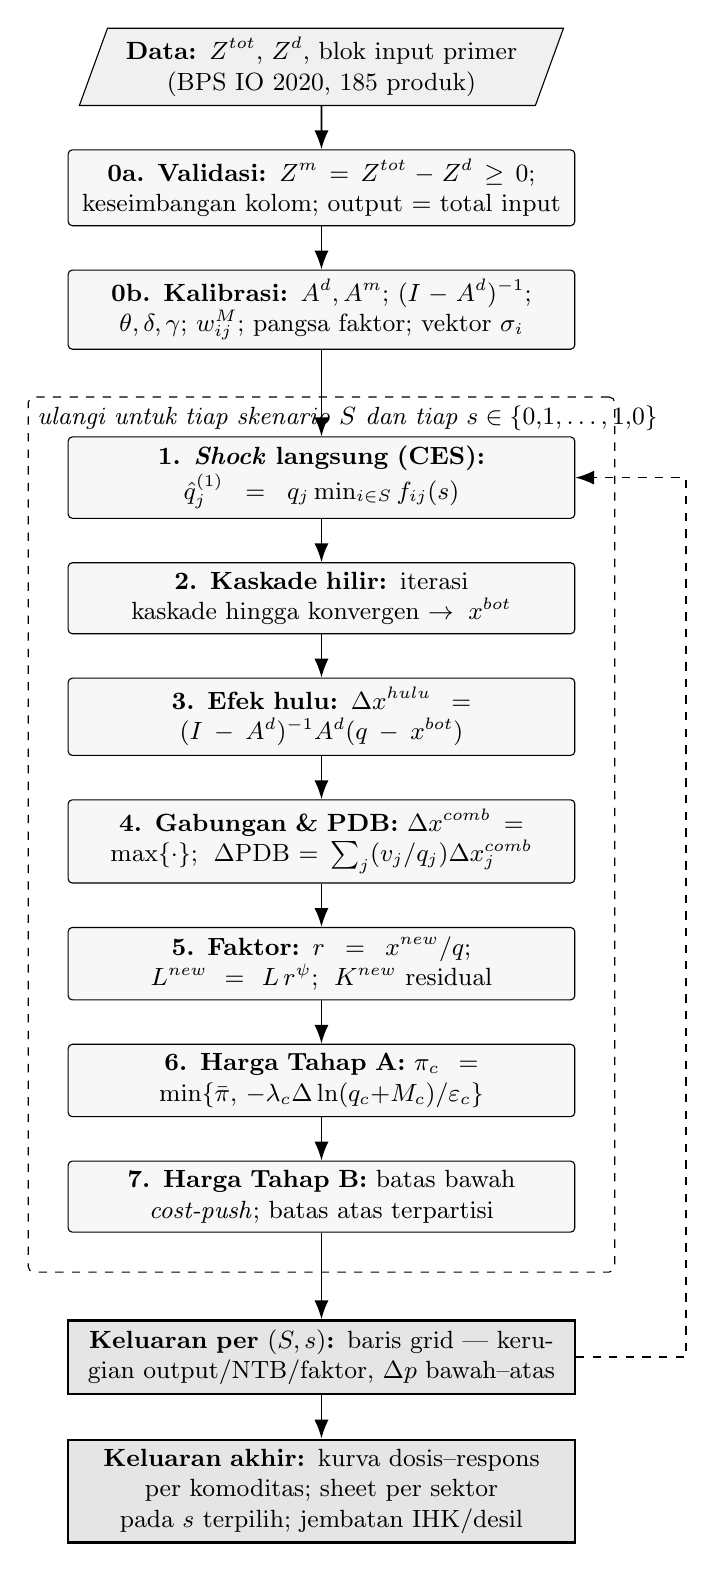
\begin{tikzpicture}[
  node distance=5.5mm and 8mm,
  font=\small,
  data/.style={trapezium, trapezium left angle=70, trapezium right angle=110,
    draw, fill=black!6, minimum height=8mm, text width=52mm, align=center},
  proc/.style={rectangle, draw, fill=black!3, rounded corners=1.5pt,
    minimum height=8mm, text width=62mm, align=center},
  outp/.style={rectangle, draw, thick, fill=black!10,
    minimum height=8mm, text width=62mm, align=center},
  loopbox/.style={rectangle, draw, dashed, inner sep=5mm, rounded corners=2pt},
  arr/.style={-{Latex[length=2.4mm]}, semithick}
]
\node[data] (dat) {\textbf{Data:} $Z^{tot}$, $Z^{d}$, blok input primer\\
  (BPS IO 2020, 185 produk)};
\node[proc, below=of dat] (val) {\textbf{0a. Validasi:} $Z^m = Z^{tot}-Z^d
  \ge 0$; keseimbangan kolom; output $=$ total input};
\node[proc, below=of val] (cal) {\textbf{0b. Kalibrasi:} $A^d, A^m$;
  $(I-A^d)^{-1}$; $\theta,\delta,\gamma$; $w^M_{ij}$;
  pangsa faktor; vektor $\sigma_i$};

\node[proc, below=11mm of cal] (l1) {\textbf{1. \en{Shock} langsung (CES):}
  $\hat q^{(1)}_j = q_j \min_{i\in S} f_{ij}(s)$};
\node[proc, below=of l1] (l2) {\textbf{2. Kaskade hilir:} iterasi kaskade
  hingga konvergen $\to x^{bot}$};
\node[proc, below=of l2] (l3) {\textbf{3. Efek hulu:}
  $\Delta x^{hulu} = (I-A^d)^{-1} A^d (q - x^{bot})$};
\node[proc, below=of l3] (comb) {\textbf{4. Gabungan \& PDB:}
  $\Delta x^{comb} = \max\{\cdot\}$;\;
  $\Delta$PDB $= \sum_j (v_j/q_j)\Delta x^{comb}_j$};
\node[proc, below=of comb] (fac) {\textbf{5. Faktor:} $r = x^{new}/q$;\;
  $L^{new} = L\, r^{\psi}$;\; $K^{new}$ residual};
\node[proc, below=of fac] (pa) {\textbf{6. Harga Tahap A:}
  $\pi_c = \min\{\bar\pi,\, -\lambda_c \Delta\ln(q_c{+}M_c)/\varepsilon_c\}$};
\node[proc, below=of pa] (pb) {\textbf{7. Harga Tahap B:} batas bawah
  \en{cost-push}; batas atas terpartisi};

\node[outp, below=11mm of pb] (grid) {\textbf{Keluaran per $(S,s)$:} baris
  grid --- kerugian output/NTB/faktor, $\Delta p$ bawah--atas};
\node[outp, below=of grid] (curve) {\textbf{Keluaran akhir:} kurva
  dosis--respons per komoditas; sheet per sektor pada $s$ terpilih;
  jembatan IHK/desil};

\draw[arr] (dat) -- (val);
\draw[arr] (val) -- (cal);
\draw[arr] (cal) -- (l1);
\draw[arr] (l1) -- (l2);
\draw[arr] (l2) -- (l3);
\draw[arr] (l3) -- (comb);
\draw[arr] (comb) -- (fac);
\draw[arr] (fac) -- (pa);
\draw[arr] (pa) -- (pb);
\draw[arr] (pb) -- (grid);
\draw[arr] (grid) -- (curve);

\begin{scope}[on background layer]
\node[loopbox, fit=(l1)(pb),
  label={[anchor=north west,font=\small\itshape]north west:
  {ulangi untuk tiap skenario $S$ dan tiap $s \in \{0{,}1,\ldots,1{,}0\}$}}]
  (loop) {};
\end{scope}
\draw[arr, dashed] (grid.east) -- ++(14mm,0) |- (l1.east);
\end{tikzpicture}%
}
\caption{Alur estimasi: dari data ke kurva dosis--respons. Kotak putus-putus
adalah loop simulasi (11 skenario $\times$ 10 titik grid $=$ 110 kombinasi).
Kalibrasi dan invers Leontief dihitung sekali di luar loop.}
\label{fig:flow}
\end{figure}

\subsection{Uraian tahap}\label{uraian-tahap}

\textbf{Tahap 0 --- persiapan (sekali, di luar loop).} (0a)
\emph{Validasi}: tiga uji identitas akuntansi (Bagian data); kegagalan
menghentikan program --- lebih baik berhenti daripada menghasilkan angka
dari data yang salah susun. (0b) \emph{Kalibrasi}: hitung \(A^d\),
\(A^m\), pangsa impor sel \(w^M_{ij}\), parameter teknologi
\(\theta, \delta, \gamma\), pangsa faktor ternormalisasi, dan --- sekali
saja, karena mahal secara komputasi --- invers Leontief
\((I - A^d)^{-1}\) yang dipakai ulang oleh Langkah 3 dan Tahap B.

\textbf{Tahap 1 --- \emph{shock} langsung.} Masukan: himpunan komoditas
\(S\), besaran \(s\), vektor \(\sigma\). Untuk tiap industri, hitung
faktor CES Persamaan~\ref{eq-cesfactor} terhadap tiap komoditas
terdampak; ambil yang terkecil. Keluaran: \(\hat q^{(1)}\), output layak
ronde pertama.

\textbf{Tahap 2 --- kaskade.} Mulai dari \(\hat q^{(1)}\), hitung rasio
ketersediaan tiap pemasok domestik; output tiap industri dibatasi
pemasok terlangkanya (yang lolos saringan \(\bar w\)) \emph{dan} batas
ronde pertamanya sendiri; ulangi sampai perubahan maksimum antar-iterasi
di bawah toleransi (\(10^{-9} \times \max q\); dalam praktik konvergen
dalam belasan iterasi). Keluaran: \(x^{bot}\).

\textbf{Tahap 3--4 --- efek hulu dan penggabungan.} Rambatkan penurunan
pembelian ke hulu lewat invers Leontief; gabungkan konservatif dengan
\(\max\); agregasi PDB dengan koefisien nilai tambah.

\textbf{Tahap 5 --- faktor.} Dari rasio output \(r\), bagi kerugian
nilai tambah menjadi kompensasi TK (dengan \emph{hoarding} \(\psi\)) dan
surplus usaha (residual, dipagari nol).

\textbf{Tahap 6--7 --- harga.} Tahap A menghitung lonjakan kelangkaan
\(\pi_c\) hanya untuk \(c \in S\); Tahap B merambatkan biaya ke 185
sektor dalam dua varian batas. Perhatikan urutannya: harga dihitung
\emph{setelah} kuantitas karena \(\Delta\ln(\text{pasokan})\) pada
Persamaan~\ref{eq-scarcity} diambil dari hasil modul kuantitas.

\textbf{Tahap 8 --- akumulasi keluaran.} Setiap kombinasi \((S, s)\)
menjadi satu baris dataset grid; rincian per 185 sektor diekspor hanya
pada \(s\) terpilih (default 0,5 dan 1,0) agar berkas hasil tetap
tertangani; kurva dosis--respons digambar dari dataset grid.

\subsection{Pseudocode}\label{pseudocode}

\begin{center}
\footnotesize
\fbox{\parbox{0.95\linewidth}{%
\textbf{Algoritme 1.} Satu kombinasi skenario $(S, s)$\par\smallskip
\begin{algorithmic}[1]
\Require $A^d, A^m, w^M, (I-A^d)^{-1}, q, v, L^{comp}, K^{sub},
         \sigma, \varepsilon, \lambda, \psi, \bar w, \bar\pi$
\State $\hat q^{(1)}_j \gets q_j \cdot \min_{i\in S} f_{ij}(s)$
       \Comment{Tahap 1: CES}
\Repeat \Comment{Tahap 2: kaskade}
  \State $\text{avail}_i \gets x_i / q_i$ untuk semua $i$
  \State $x_j \gets q_j \cdot \min\bigl\{\hat q^{(1)}_j/q_j,\;
         \min_{i:\,a^d_{ij}>\bar w} [1 - a^d_{ij}(1-\text{avail}_i)]
         \bigr\}$ \Comment{proporsional; strict: ganti dgn avail$_i$}
\Until{$\max_j |\Delta x_j| < \text{tol}\cdot\max(q)$}
\State $\Delta x^{hulu} \gets (I-A^d)^{-1} A^d (q - x)$
       \Comment{Tahap 3}
\State $\Delta x^{comb} \gets \max\{(q-\hat q^{(1)}) + (\hat q^{(1)}-x),\;
       \Delta x^{hulu}\}$ per sektor \Comment{Tahap 4}
\State $\Delta\text{PDB} \gets \sum_j (v_j/q_j)\,\Delta x^{comb}_j$
\State $r \gets 1 - \Delta x^{comb} \oslash q$;\quad
       $L^{new} \gets L^{comp} \odot r^{\psi}$
       \Comment{Tahap 5}
\State $K^{new} \gets \max\{0,\; r\odot(L^{comp}{+}K^{sub}) - L^{new}\}$
\ForAll{$c \in S$} \Comment{Tahap 6: harga kelangkaan}
  \State $\pi_c \gets \min\bigl\{\bar\pi,\;
         -\lambda_c\,\Delta\ln(q_c + M_c)\,/\,\varepsilon_c\bigr\}$
\EndFor
\State $\Delta p^{bawah} \gets (I - A^{d\prime})^{-1} A^{m\prime}\,
       \Delta p_m$ \Comment{Tahap 7}
\State $\Delta p^{atas}_N \gets (I - A^{d\prime}_{NN})^{-1}
       A^{tot\prime}_{SN}\, \pi_S$; \quad $\Delta p^{atas}_S \gets \pi_S$
\State \Return baris grid: $\Delta x^{comb}, \Delta\text{PDB},
       \Delta L, \Delta K, \Delta p^{bawah}, \Delta p^{atas}$
\end{algorithmic}
}}
\end{center}

\section{Hasil Simulasi}\label{sec-hasil}

Tabel~\ref{tbl-hasil} merangkum hasil pada \emph{shock} moderat
(\(s = 0{,}1\)) dan berat (\(s =
0{,}5\)); nilai hingga \(s = 1\) terbaca pada Gambar~\ref{fig-dosis};
kurva dosis--respons lengkap tersedia pada berkas keluaran. Seluruh
angka memakai parameter baseline (Tabel~\ref{tab:param}) --- termasuk
pengecualian sel terkontaminasi produk 9 \(\to\) industri Minyak Nabati
(\texttt{SHOCK\_EXEMPT}; lihat Bagian~\ref{sec-param}) --- dan dibaca
\emph{per periode disrupsi}; kisaran ketidakpastiannya diberikan oleh
\emph{robustness test} (Bagian~\ref{sec-robust}).

\begin{longtable}[]{@{}
  >{\raggedright\arraybackslash}p{(\linewidth - 10\tabcolsep) * \real{0.2857}}
  >{\centering\arraybackslash}p{(\linewidth - 10\tabcolsep) * \real{0.1429}}
  >{\centering\arraybackslash}p{(\linewidth - 10\tabcolsep) * \real{0.1429}}
  >{\centering\arraybackslash}p{(\linewidth - 10\tabcolsep) * \real{0.1429}}
  >{\centering\arraybackslash}p{(\linewidth - 10\tabcolsep) * \real{0.1429}}
  >{\centering\arraybackslash}p{(\linewidth - 10\tabcolsep) * \real{0.1429}}@{}}
\caption{Hasil baseline: kerugian NTB (\% PDB), lonjakan harga komoditas
terdampak (\%), dan indeks harga produsen tertimbang output batas atas
(\%). Tanda † = lonjakan harga terpangkas plafon \(\bar\pi\)
(\(+172\%\)).}\label{tbl-hasil}\tabularnewline
\toprule\noalign{}
\begin{minipage}[b]{\linewidth}\raggedright
Skenario
\end{minipage} & \begin{minipage}[b]{\linewidth}\centering
NTB \%PDB (s=0,1)
\end{minipage} & \begin{minipage}[b]{\linewidth}\centering
NTB \%PDB (s=0,5)
\end{minipage} & \begin{minipage}[b]{\linewidth}\centering
Harga \% (s=0,1)
\end{minipage} & \begin{minipage}[b]{\linewidth}\centering
Harga \% (s=0,5)
\end{minipage} & \begin{minipage}[b]{\linewidth}\centering
Indeks harga atas (s=0,5)
\end{minipage} \\
\midrule\noalign{}
\endfirsthead
\toprule\noalign{}
\begin{minipage}[b]{\linewidth}\raggedright
Skenario
\end{minipage} & \begin{minipage}[b]{\linewidth}\centering
NTB \%PDB (s=0,1)
\end{minipage} & \begin{minipage}[b]{\linewidth}\centering
NTB \%PDB (s=0,5)
\end{minipage} & \begin{minipage}[b]{\linewidth}\centering
Harga \% (s=0,1)
\end{minipage} & \begin{minipage}[b]{\linewidth}\centering
Harga \% (s=0,5)
\end{minipage} & \begin{minipage}[b]{\linewidth}\centering
Indeks harga atas (s=0,5)
\end{minipage} \\
\midrule\noalign{}
\endhead
\bottomrule\noalign{}
\endlastfoot
Gula (65) & 0,39 & 2,17 & 8 & 50 & 0,24 \\
Tepung dst (61) & 0,26 & 1,47 & 6 & 35 & 0,10 \\
Kakao (23) & 0,08 & 0,44 & 2 & 10 & 0,04 \\
Gandum (9) & 0,05 & 0,27 & 35 & 172† & 0,26 \\
Kedelai (7) & 0,05 & 0,26 & 31 & 172† & 0,09 \\
Olahan buah-sayur (57) & 0,02 & 0,11 & 4 & 22 & 0,04 \\
Garam (50) & 0,01 & 0,07 & 13 & 92 & 0,02 \\
\textbf{Bundel (7 komoditas)} & \textbf{0,48} & \textbf{2,64} & 35 &
172† & 0,75 \\
\end{longtable}

\subsection{Cara membaca hasil utama}\label{cara-membaca-hasil-utama}

\textbf{Gula memimpin; gandum menemukan bentuk aslinya.} Setelah
dekontaminasi produk 9 (pengecualian sel Minyak Nabati), peringkat
kuantitas dipimpin \textbf{gula} pada semua \(s\) --- pola ``eksposur
langsung terluas'' yang terus terakumulasi --- disusul tepung dan kakao.
\textbf{Gandum} turun ke jejak PDB yang moderat (0,27\% pada
\(s = 0{,}5\)), tetapi itu justru bentuk aslinya: dampaknya
\emph{terkonsentrasi} pada satu rantai (penggilingan terigu kehilangan
sekitar separuh output; harga produsen terigu \textbf{+89\%}) dan
karenanya bergeser klasifikasi --- dari komoditas risiko-output menjadi,
bersama kedelai, komoditas \emph{risiko-harga rantai-spesifik}: kecil di
agregat PDB, memaku plafon harga sejak \(s = 0{,}5\), dengan transmisi
langsung ke harga pangan pokok (mie, roti).

\textbf{Kelompok risiko-harga: gandum, kedelai, garam.} Ketiganya kecil
pada kolom kuantitas tetapi memaku plafon harga: gandum dan kedelai
sejak \(s = 0{,}5\) (yang terakhir konsisten dengan episode tempe 2022),
garam pada \emph{shock} berat. Profil ini --- ditambah catatan salensi
distribusional kedelai (Bagian~\ref{sec-screening}) --- berarti keduanya
masuk pembahasan kebijakan lewat pintu harga konsumen, bukan pintu PDB.

\textbf{Pola faktor.} Pada semua skenario, kerugian surplus usaha (\%)
\(>\) kerugian output \(>\) kerugian kompensasi TK --- mekanika
\emph{labor hoarding} bekerja sesuai desain: upah turun lebih lambat
dari output dan selisihnya ditanggung laba (dan pendapatan usaha rumah
tangga, pada sektor pertanian/informal).

\textbf{Bundel sub-aditif.} Kerugian bundel (2,64\%) melebihi setiap
komponen tetapi di bawah jumlah komponennya --- tumpang tindih jalur
kaskade dan aturan min antar komoditas bekerja sebagaimana mestinya.

\begin{figure}[htbp!]

\centering{

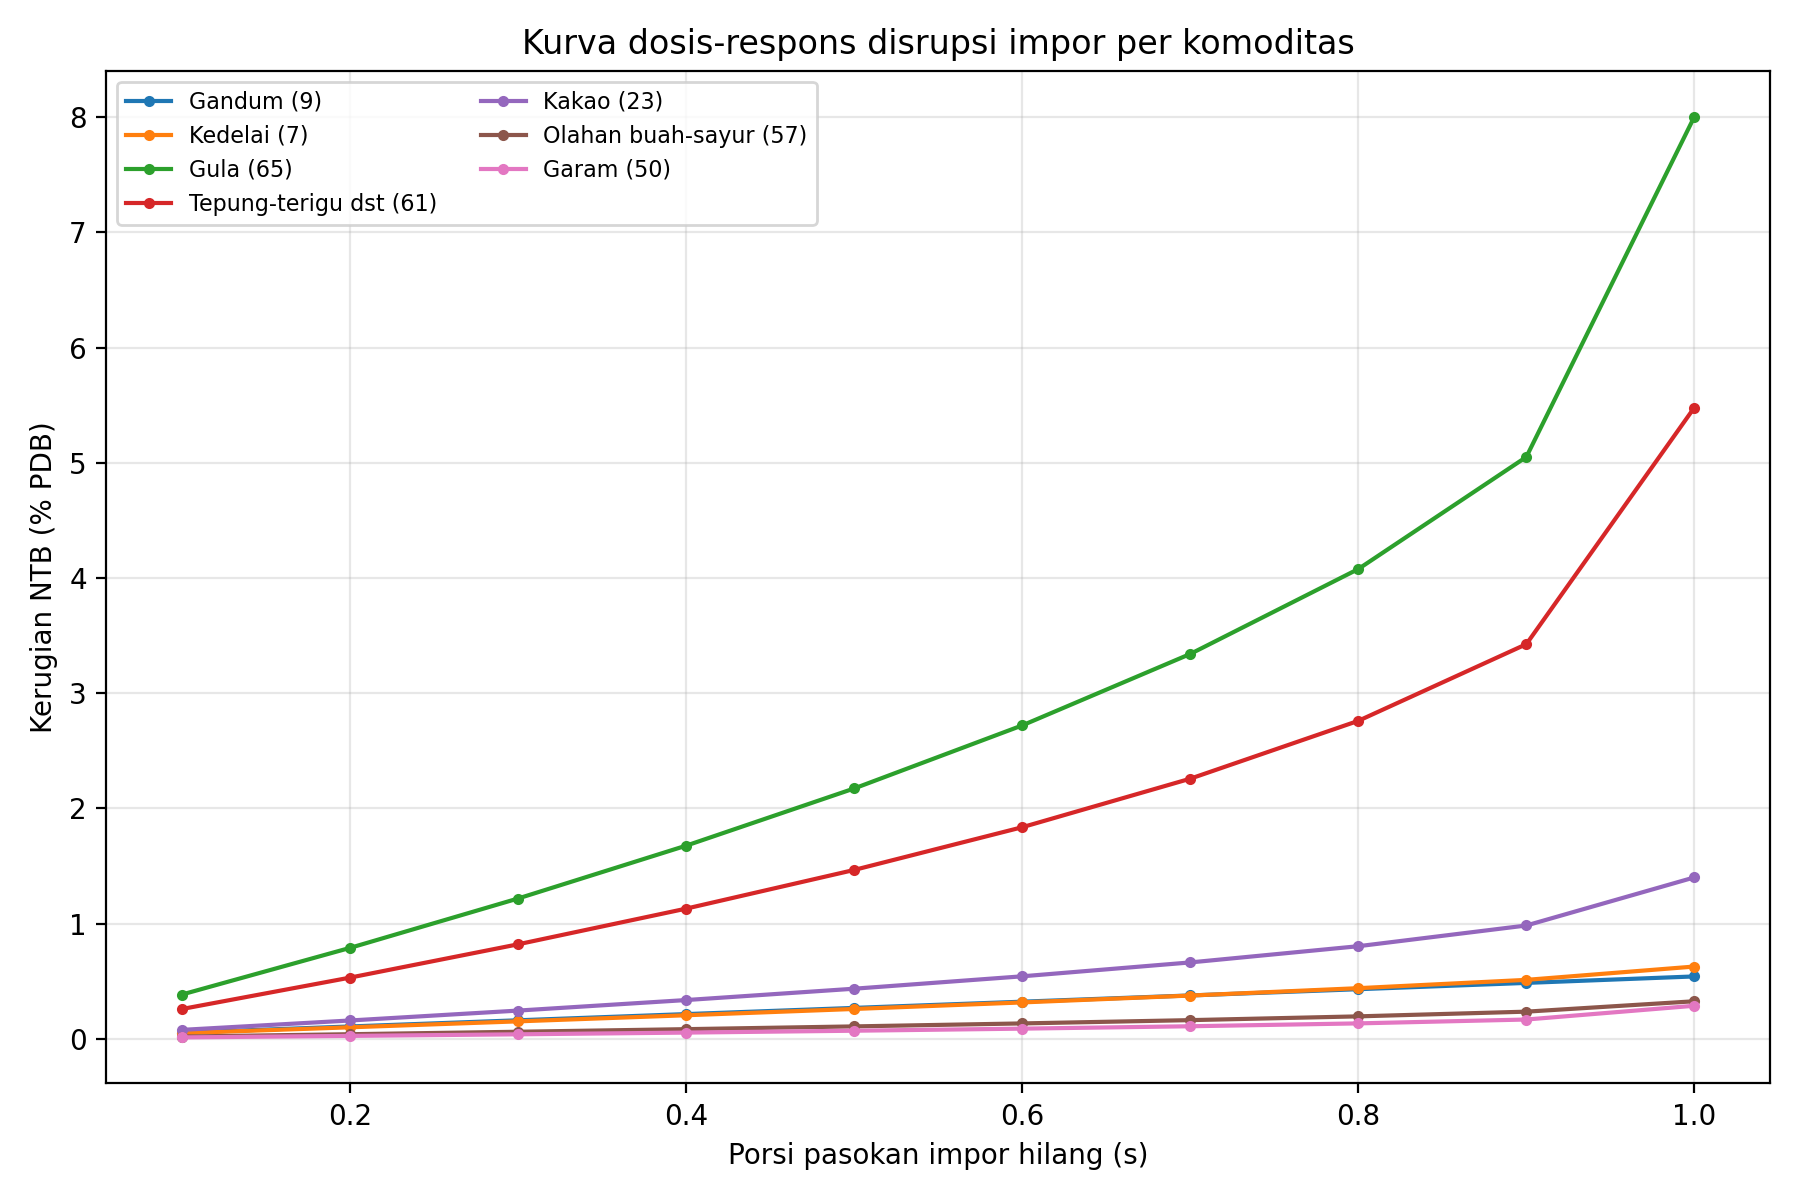
\includegraphics[width=0.92\linewidth,height=\textheight,keepaspectratio]{data/interim/dosis_respons_komoditas.png}

}

\caption{\label{fig-dosis}Kurva dosis--respons: kerugian NTB (\% PDB)
terhadap besaran \emph{shock} \(s\), per skenario (baseline). Kemiringan
awal mencerminkan eksposur impor; kelengkungan menjelang \(s = 1\)
mencerminkan esensialitas (\(\sigma\)).}

\end{figure}%

\subsection{Rincian: industri yang paling
terdampak}\label{rincian-industri-yang-paling-terdampak}

Uraian berikut merinci lima industri dengan kerugian NTB terbesar pada
tiga skenario teratas (\(s = 0{,}5\)).

\emph{(Catatan produksi: gambar ``lima industri paling terdampak per
skenario pada \(s =
0{,}5\)'' belum disertakan --- berkas \texttt{fig\_top\_industri.png}
perlu digenerasi dari \texttt{code/simulasi\_disrupsi\_impor.py}, lalu
sisipan gambar di bawah tinggal diaktifkan.)}

\textbf{Gandum (9): rantai terigu, pasca-dekontaminasi.} Versi awal
skenario ini menghasilkan absurditas yang instruktif: industri paling
terdampak adalah Minyak Nabati dan, lewat efek hulu, Kelapa Sawit ---
padahal tidak ada kilang minyak yang membeli gandum. Penelusuran sel
menunjukkan produk 9 (kategori residual ``padi-padian \emph{dan bahan
makanan lainnya}'') memuat bahan baku impor industri minyak makan yang
bukan gandum; sel (9 \(\to\) Minyak Nabati) kemudian \emph{dikecualikan
dari shock} melalui mekanisme \texttt{SHOCK\_EXEMPT} (terdokumentasi di
registri parameter). Pasca-koreksi, gambar gandum menjadi bersih dan
sesuai ekonomi: kerugian terkonsentrasi di \textbf{Tepung Terigu \&
Pati} dan \textbf{Tepung Lainnya} (masing-masing \(\approx -\)Rp
5,6--5,9 T NTB) dengan harga produsen terigu \textbf{+89\%} pada \(s =
0{,}5\); \emph{Ubi Kayu} terseret lewat efek permintaan hulu (industri
tepung yang terkendala membeli lebih sedikit tapioka); dan \emph{Minuman
Beralkohol} terkena langsung (harga +30\%) --- jejak
\textbf{malt/barley}, isi non-gandum produk 9 yang \emph{memang benar}
biji-bijian impor dan karena itu dipertahankan dalam \emph{shock}.
Episode ini sekaligus pelajaran metodologis: hasil yang janggal bagi
pembaca yang paham ekonominya adalah alat validasi --- persis peran
lapisan pakar pada tabel kritikalitas. Satu inkonsistensi kecil yang
disadari: sisi harga (Tahap B) masih merambatkan kenaikan harga produk 9
ke seluruh pengguna termasuk sel yang dikecualikan; efeknya kecil dan
konservatif, dan akan dirapikan bersama pemisahan penuh produk 9.

\textbf{Gula (65): keluasan yang terkonfirmasi di tingkat industri.}
Lima teratas mencakup empat kanal berbeda: jasa makanan (Penyediaan
Makan-Minum, \(-\)Rp 81 T --- pengguna gula langsung terbesar), industri
makanan olahan (Makanan Lainnya), produk susu, dan Minuman Non-Alkohol
(kenaikan harga produsen +5,8\%); Perdagangan terseret lewat efek
permintaan. Tidak ada satu rantai yang dominan --- persis pola
``eksposur langsung terluas'' yang menjelaskan mengapa gula terus
terakumulasi hingga menyalip gandum pada \(s = 1\).

\textbf{Tepung dst. (61): jasa makanan, roti, dan jejak ke hulu.}
Penyediaan Makan-Minum kembali teratas (\(-\)Rp 77 T), disusul Roti \&
Biskuit (harga +2,3\%) dan --- karena produk 61 juga memuat tepung beras
--- efek permintaan hulu yang menjalar sampai Penggilingan Padi dan
\emph{Padi} (\(-\)Rp 13 T di tingkat usaha tani): disrupsi impor tepung
menurunkan permintaan turunan terhadap gabah domestik. Pakan Olahan juga
masuk lima besar, mengonfirmasi tautan tepung--pakan.

\textbf{Satu pola lintas skenario.} Penyediaan Makan dan Minum masuk
lima besar pada \emph{ketiga} skenario --- sektor jasa makanan adalah
titik konvergensi hilir sistem pangan, sehingga menjadi kandidat alami
indikator pemantauan tunggal untuk disrupsi pangan apa pun.

\section{Robustness Test}\label{sec-robust}

\subsection{Desain}\label{desain}

Dua belas varian \emph{one-at-a-time} di sekitar baseline: ambang
saringan \(\bar w \in
\{0{,}01^*; 0{,}03; 0{,}05\}\); skala \(\sigma\)
\(\{{\times}0{,}5; {\times}1^*;
{\times}2\}\); \(\psi \in \{0{,}5; 0{,}7^*; 1{,}0\}\); skala
\(\varepsilon\) \(\{{\times}0{,}5; {\times}1^*; {\times}1{,}5\}\);
\(\lambda \in \{0{,}5; 1{,}0^*\}\); ditambah dua varian khusus:
\emph{substitusi sempurna} (\(\sigma = 999\); spesifikasi awal) dan
\emph{kaskade ketat} (batas atas teoretis). Setiap varian menjalankan
seluruh skenario; stabilitas peringkat diukur dengan korelasi Spearman
terhadap baseline pada \(s = 0{,}5\).

\subsection{Hasil}\label{hasil}

\begin{longtable}[]{@{}lcc@{}}
\caption{\emph{Robustness test} (konfigurasi terkini, termasuk
\texttt{SHOCK\_EXEMPT}): kerugian NTB bundel pada \(s = 0{,}5\) dan
korelasi peringkat Spearman terhadap baseline (7
komoditas).}\label{tbl-robust}\tabularnewline
\toprule\noalign{}
Varian & Bundel (\% PDB) & Spearman \\
\midrule\noalign{}
\endfirsthead
\toprule\noalign{}
Varian & Bundel (\% PDB) & Spearman \\
\midrule\noalign{}
\endhead
\bottomrule\noalign{}
\endlastfoot
baseline & 2,64 & 1,000 \\
\(\bar w = 0{,}03\) & 0,88 & 0,643 \\
\(\bar w = 0{,}05\) & 0,67 & 0,714 \\
\(\sigma \times 0{,}5\) & 2,99 & 0,964 \\
\(\sigma \times 2\) & 2,48 & 1,000 \\
\(\psi = 0{,}5\) / \(1{,}0\) & 2,64 & 1,000 \\
\(\varepsilon \times 0{,}5\) / \(\times 1{,}5\) & 2,64 & 1,000 \\
\(\lambda = 0{,}5\) & 2,64 & 1,000 \\
substitusi sempurna & 2,33 & 1,000 \\
kaskade ketat & 55,41 & 0,321 \\
tanpa-\emph{exempt} (9\$\to\$58) & 4,71 & 0,786 \\
\end{longtable}

Empat temuan:

\begin{enumerate}
\def\labelenumi{\arabic{enumi}.}
\tightlist
\item
  \textbf{Anggaran ketidakpastian dimiliki oleh pilihan transmisi
  jaringan, bukan parameter perilaku.} Menggandakan atau membagi dua
  \(\sigma\) hanya menggeser bundel pada 2,3--3,0\%; \(\psi\),
  \(\varepsilon\), \(\lambda\) tidak menyentuh kuantitas menurut
  konstruksi. Sebaliknya, menaikkan \(\bar w\) dari 0,01 ke 0,03
  memangkas bundel dari 2,64\% menjadi 0,88\% --- sebagian besar
  estimasi baseline merambat lewat tautan berpangsa biaya 1--3\%.
  Kisaran sentral yang jujur: \textbf{0,7--2,6\% PDB} (bundel,
  \(s = 0{,}5\)), dengan batas atas teoretis 55\% (kaskade ketat,
  lampiran).
\item
  \textbf{Koreksi dekontaminasi terukur besarnya.} Varian
  tanpa-\emph{exempt} mereproduksi persis konfigurasi pra-koreksi:
  bundel 4,71\% --- sel (9 \(\to\) Minyak Nabati) sendirian menyumbang
  2,07 poin persentase PDB (44\% dari angka utama lama) dan menggeser
  peringkat (Spearman 0,786). Pengecualian sel bukan penyetelan
  kosmetik, melainkan koreksi material yang kini terkuantifikasi.
\item
  \textbf{Kestabilan peringkat berbentuk keanggotaan kelompok --- dengan
  batas yang kini lebih tegas.} Yang stabil pada seluruh varian sentral:
  \emph{gula pada peringkat 1}, serta ekor \{olahan buah-sayur, garam\}
  pada peringkat 6--7 (garam peringkat 7 di \emph{setiap} varian,
  termasuk kaskade ketat). Kelompok tengah (tepung, kakao, gandum,
  kedelai) \emph{menyusun ulang urutannya} mengikuti \(\bar w\): tepung
  turun (2 \(\to\) 5) dan gandum--kedelai naik ketika ambang dinaikkan
  --- rantai tepung berjalan lewat tautan berpangsa 1--3\%, rantai
  gandum--kedelai lewat tautan dalam yang lolos ambang berapa pun.
  Kaskade ketat mengacak peringkat secara drastis (Spearman 0,321),
  memperkuat statusnya sebagai batas atas lampiran, bukan spesifikasi.
\item
  \textbf{Implikasi prioritas kerja.} Urutan kelompok tengah bergantung
  sepenuhnya pada pertanyaan ``apakah tautan 1--3\% menularkan
  \emph{shock}?'' --- persis pertanyaan yang dijawab tabel kritikalitas
  level-pasangan (Bagian~\ref{sec-ext}): terigu ke mie jelas menularkan;
  tautan insidental 1,5\% tidak. \emph{Robustness test} dengan demikian
  memprioritaskan sendiri sisa rencana kerja: tabel kritikalitas naik ke
  urutan teratas bersama kalibrasi historis.
\end{enumerate}

\section{Registri Parameter dan Asumsi}\label{sec-param}

Tabel~\ref{tab:param} (halaman \emph{landscape} berikut) merangkum
seluruh parameter yang \emph{diasumsikan}, dikelompokkan menurut
pengaruhnya pada hasil, disertai basis dan arah bias. Kejujuran yang
perlu dinyatakan di muka: parameter Tier 1 --- yang paling menentukan
hasil --- belum memiliki basis empiris Indonesia yang dapat dikutip.
Rencana pemutakhirannya dirinci pada Bagian~\ref{sec-ext}; hingga saat
itu, seluruh angka level dibaca sebagai kisaran indikatif, sementara
\emph{peringkat} antarkomoditas sudah dapat diandalkan.

\begin{landscape}
\begin{longtable}{@{}p{3.6cm}p{3.6cm}p{6.5cm}p{7.5cm}@{}}
\caption{Registri parameter dan asumsi.}
\label{tab:param}\\
\toprule
\textbf{Parameter} & \textbf{Nilai saat ini} & \textbf{Basis} &
\textbf{Peran / arah bias} \\
\midrule
\endfirsthead
\multicolumn{4}{@{}l}{\emph{(lanjutan Tabel~\ref{tab:param})}}\\
\toprule
\textbf{Parameter} & \textbf{Nilai saat ini} & \textbf{Basis} &
\textbf{Peran / arah bias} \\
\midrule
\endhead
\multicolumn{4}{@{}l}{\emph{Tier 1 --- penggerak hasil utama}}\\
\addlinespace[2pt]
$\sigma_i$ --- elastisitas CES domestik--impor per komoditas &
default 2{,}0; jagung 3{,}0; garam 1{,}3; sapi, susu, tepung, gula, pakan
1{,}5; lainnya 2{,}0 &
Pertimbangan analis berjangkar aturan praktis ``setengah elastisitas
Armington GTAP''; belum ada variasi per pasangan komoditas--industri &
Parameter paling menentukan, khususnya menjelang $s = 1$; mengatur
kelengkungan kurva dosis--respons dan ambang esensialitas (industri
berhenti total bila $\sigma \le 1$ pada $s = 1$) \\
\addlinespace[3pt]
$\bar w$ --- ambang pangsa biaya (\texttt{critshare}), berlaku di
Langkah 1 \emph{dan} 2 &
0{,}01 (sensitivitas 0{,}03; 0{,}05) &
\en{Robustness test} data riil (uji robustness): bundel 2{,}64\% $\to$
0{,}88\% saat $\bar w$ 0{,}01 $\to$ 0{,}03 --- parameter paling
menggerakkan besaran; puncak dan ekor peringkat tetap stabil &
Ambang berapa pun salah-klasifikasi input murah-tapi-esensial (karagenan;
garam utk klor-alkali) --- motivasi tabel kritikalitas pada ekstensi \\
\addlinespace[3pt]
\texttt{SHOCK\_EXEMPT} --- pengecualian sel terkontaminasi &
$\{9 \to 58\}$ (Minyak Nabati) &
Penelusuran sel: pembelian produk 9 oleh industri minyak berpangsa impor
tinggi tetapi bukan gandum (kategori residual) &
Tanpa pengecualian, skenario gandum salah menghantam rantai sawit;
kandidat pengecualian baru wajib diverifikasi sel per sel \\
\addlinespace[3pt]
Aturan transmisi kaskade (\texttt{CASCADE\_STRICT}) &
Proporsional: $c_{ij} = 1 - a^d_{ij}(1 - \text{avail}_i)$ &
Gaya Hallegatte/ARIO; aturan ketat (min murni) menular tanpa peredaman
lewat sektor hub (perdagangan, listrik) pada data riil &
Ketat dilaporkan hanya sbg batas atas teoretis di lampiran; pasangan
benar-benar esensial dikembalikan ke min lewat tabel kritikalitas \\
\addlinespace[3pt]
$\psi$ --- \en{labor hoarding} &
0{,}7 &
Penalaran gaya hukum Okun jangka pendek; belum diestimasi dari data
Indonesia &
Menskalakan seluruh kerugian upah dan \en{headcount}; selisihnya
ditanggung surplus usaha sebagai residual \\
\addlinespace[3pt]
$\varepsilon_c$ --- elastisitas permintaan jangka pendek &
0{,}30--0{,}60 per produk (pangan pokok rendah; olahan lebih tinggi) &
Kisaran literatur permintaan pangan Indonesia (estimasi gaya Deaton pada
Susenas); belum disumberkan pada estimasi spesifik &
Lonjakan harga kelangkaan $\propto 1/\varepsilon$; kesalahan dua kali
lipat pada $\varepsilon$ berarti kesalahan dua kali lipat pada angka
harga utama \\
\addlinespace[5pt]
\multicolumn{4}{@{}l}{\emph{Tier 2 --- saklar struktural/perilaku}}\\
\addlinespace[2pt]
$\lambda_c$ --- porsi penyelesaian lewat harga &
1{,}0 &
Pasar pangan terbuka; penjatahan non-harga diabaikan &
Menskalakan Tahap A secara linear \\
$\bar\pi$ --- plafon kenaikan harga &
1{,}0 log poin ($\approx +172\%$) &
Pagar pengaman terhadap ledakan numerik &
Arbitrer; setiap pelanggaran dicetak sebagai sinyal pasar tipis \\
Aturan penjatahan kaskade &
Proporsional terhadap pembelian normal &
Konvensi netral &
Alternatif penjatahan prioritas (pangan sebelum pakan) belum
diimplementasi \\
Aturan penggabungan pasokan--permintaan &
$\max$ per sektor &
Konvensi konservatif &
Menghindari penghitungan ganda tumpang tindih dua arah rambatan \\
Pasokan domestik komoditas terdampak &
Tetap (tidak dapat bertambah) &
Horizon pendek &
Mengabaikan kapasitas menganggur (mis.\ rafinasi gula) \\
Persediaan \& pengalihan asal impor &
Nol &
Belum diimplementasi (lihat ekstensi) &
Setiap skenario adalah kasus tanpa peringatan dan tanpa stok $\Rightarrow$
membesarkan estimasi \\
Penutupan Type I &
Permintaan akhir beku &
Pilihan desain &
Mengecilkan estimasi; kerugian pendapatan dihitung tetapi tidak
diumpanbalikkan \\
\en{Pass-through} dan margin &
Penuh; margin per unit tetap &
Struktur dual Leontief &
Batas atas transmisi harga ke konsumen \\
\addlinespace[5pt]
\multicolumn{4}{@{}l}{\emph{Tier 3 --- konvensi kalibrasi}}\\
\addlinespace[2pt]
Teknologi $A, \gamma, \theta, \delta$ &
Tetap pada nilai IO 2020 &
Definisi jangka pendek &
--- \\
Efisiensi \en{benchmark} &
$\theta VA = \delta M = Q$ &
Implikasi langsung kalibrasi &
Pengurangan material apa pun langsung mengikat output \\
Residual NTB (penyusutan dll.) &
Proporsional terhadap output &
Pelengkap normalisasi pangsa faktor &
--- \\
Ukuran kekurangan pada model harga &
$s\,M_c/(q_c + M_c)$; $M$ hanya impor antara &
Keterbatasan data (matriks impor permintaan akhir tidak dimuat) &
Mengecilkan kekurangan untuk komoditas yang impornya dominan ke konsumsi
akhir (mis.\ susu); ekspor diabaikan pada penyebut \\
Pemetaan komoditas--produk &
Tabel pemetaan komoditas &
Konkordansi manual &
Bias terdokumentasi per baris (bungkil kecil; karagenan besar) \\
Numerik &
Toleransi $10^{-9}$; maksimum 500 iterasi &
--- &
Tidak material \\
\bottomrule
\end{longtable}
\end{landscape}

\section{Asumsi yang Mendasari Keseluruhan Simulasi}\label{sec-asumsi}

Bagian ini merangkum asumsi \emph{struktural} yang mendasari seluruh
simulasi --- yaitu pilihan tentang cara ekonomi bekerja, bukan nilai
parameter (nilai parameter dirangkum terpisah pada
Tabel~\ref{tab:param}). Setiap asumsi disertai maknanya dalam bahasa
sederhana dan arah biasnya terhadap hasil.

\subsection{Asumsi teknologi dan
produksi}\label{asumsi-teknologi-dan-produksi}

\begin{enumerate}
\def\labelenumi{\arabic{enumi}.}
\tightlist
\item
  \textbf{Resep produksi tetap.} Koefisien input--output (\(A\),
  \(\gamma\), \(\theta\), \(\delta\)) dibekukan pada nilai Tabel IO
  2020. Maknanya: dalam horizon simulasi, tidak ada industri yang sempat
  mengubah teknologi, mengganti bahan baku dengan bahan lain, atau
  berinvestasi pada proses baru. Asumsi ini masuk akal untuk hitungan
  minggu sampai sekitar dua triwulan, dan menjadi makin tidak realistis
  untuk horizon yang lebih panjang. Arah bias: \emph{membesarkan}
  kerugian.
\item
  \textbf{Tidak ada kapasitas menganggur pada kondisi awal.} Kalibrasi
  menyiratkan kedua cabang fungsi produksi tepat mengikat
  (\(\theta VA = \delta M = Q\)), sehingga setiap pengurangan bahan baku
  langsung memotong output --- tidak ada ``ruang gerak'' berupa mesin
  atau pekerja yang selama ini setengah menganggur. Arah bias:
  \emph{membesarkan} kerugian.
\item
  \textbf{Pasokan domestik komoditas terdampak tidak dapat bertambah.}
  Petani jagung tidak dapat mempercepat panen; pabrik garam tidak dapat
  menambah produksi dalam hitungan minggu. Kapasitas menganggur yang
  mungkin ada (misalnya rafinasi gula) diabaikan. Arah bias:
  \emph{membesarkan} kerugian.
\item
  \textbf{Substitusi hanya antara varietas domestik dan impor dari
  produk yang sama} (melalui CES, Bagian~\ref{sec-ces}). Tidak ada
  substitusi \emph{antarproduk}: rumah makan tidak beralih dari ayam ke
  ikan, pabrik roti tidak beralih dari terigu ke tepung lain. Arah bias:
  \emph{membesarkan} kerugian.
\end{enumerate}

\subsection{\texorpdfstring{Asumsi tentang
\emph{shock}}{Asumsi tentang shock}}\label{asumsi-tentang-shock}

\begin{enumerate}
\def\labelenumi{\arabic{enumi}.}
\setcounter{enumi}{4}
\tightlist
\item
  \textbf{\emph{Shock} datang tanpa peringatan dan tanpa penyangga.}
  Tidak ada stok bahan baku, tidak ada pengalihan ke negara pemasok
  lain, tidak ada pembelian antisipatif. Setiap skenario adalah kasus
  terburuk dari sisi kesiapan. Arah bias: \emph{membesarkan} kerugian
  (ekstensi penyangga direncanakan, Bagian~\ref{sec-ext}).
\item
  \textbf{Pasokan yang tersisa dijatah proporsional.} Impor yang masih
  masuk dibagi ke pengguna sebanding dengan pembelian normalnya; tidak
  ada prioritas (misalnya pangan didahulukan daripada pakan) dan tidak
  ada perebutan lewat harga. Arah bias: netral terhadap total, tetapi
  memengaruhi \emph{distribusi} kerugian antarindustri.
\item
  \textbf{Durasi tidak dimodelkan secara eksplisit.} Hasil berlaku untuk
  ``satu periode disrupsi''; kerugian rupiah harus dibaca per satuan
  durasi episode yang diasumsikan pembaca.
\end{enumerate}

\subsection{Asumsi pasar dan perilaku}\label{asumsi-pasar-dan-perilaku}

\begin{enumerate}
\def\labelenumi{\arabic{enumi}.}
\setcounter{enumi}{7}
\tightlist
\item
  \textbf{Permintaan akhir beku (penutupan Type I).} Rumah tangga,
  pemerintah, dan ekspor tetap meminta jumlah yang sama; kerugian
  pendapatan pekerja dan pengusaha (yang dihitung di
  Bagian~\ref{sec-factor}) tidak diumpanbalikkan menjadi penurunan
  belanja. Arah bias: \emph{mengecilkan} kerugian total.
\item
  \textbf{Kebutuhan nilai tambah turun sebanding output}, dan
  pembagiannya antara upah dan surplus mengikuti aturan \emph{hoarding}:
  pekerjaan turun lebih lambat daripada output, selisihnya ditanggung
  laba (Bagian~\ref{sec-factor}). Tidak ada PHK massal seketika, tetapi
  juga tidak ada perekrutan.
\item
  \textbf{Tidak ada respons kebijakan.} Pemerintah tidak melakukan
  operasi pasar, tidak melepas cadangan, tidak memberi subsidi. Hasil
  simulasi adalah dampak ``tanpa intervensi'' --- justru berguna sebagai
  pembanding untuk menilai seberapa besar intervensi yang dibutuhkan.
\end{enumerate}

\subsection{Asumsi sisi harga}\label{asumsi-sisi-harga}

\begin{enumerate}
\def\labelenumi{\arabic{enumi}.}
\setcounter{enumi}{10}
\tightlist
\item
  \textbf{Kelangkaan diselesaikan lewat harga} (porsi \(\lambda_c\)):
  harga komoditas terdampak naik sampai permintaan menyamai pasokan yang
  tersisa; kurva permintaan tidak bergeser (tidak ada panik atau
  penimbunan oleh konsumen). Arah bias: pada episode krisis nyata, panik
  justru menggeser permintaan ke atas, sehingga asumsi ini cenderung
  \emph{mengecilkan} lonjakan harga.
\item
  \textbf{Rente kelangkaan berhenti di tingkat komoditas.} Industri
  hilir tidak menambah margin; mereka hanya meneruskan kenaikan biaya
  secara penuh dengan margin per unit tetap (\emph{full pass-through}).
  Kombinasinya menjadikan varian ``batas atas'' Tahap B sebagai plafon
  transmisi harga, dan varian ``batas bawah'' sebagai lantainya.
\item
  \textbf{Modul kuantitas dan modul harga memakai \emph{shock} dan
  parameter substitusi yang sama} (\(s\) dan \(\sigma\)), sehingga angka
  kuantitas dan harga dalam satu laporan konsisten satu sama lain ---
  tetapi keduanya tetap dihitung terpisah, tanpa umpan balik harga ke
  kuantitas (bukan keseimbangan umum).
\end{enumerate}

Ringkasnya: sebagian besar asumsi produksi dan \emph{shock} condong
\emph{membesarkan} estimasi kerugian, sedangkan pembekuan permintaan
akhir condong \emph{mengecilkannya}. Keduanya tidak saling menghapus
secara otomatis; karena itulah hasil disajikan sebagai kisaran, dan
\emph{peringkat} antarkomoditas --- yang stabil terhadap semua variasi
ini --- diperlakukan sebagai keluaran utama.

\section{Keterbatasan}\label{sec-limit}

\begin{enumerate}
\def\labelenumi{\arabic{enumi}.}
\tightlist
\item
  \textbf{Bukan keseimbangan umum.} Harga dan kuantitas tidak ditentukan
  bersama; tidak ada klaim kesejahteraan. Modul kuantitas menjawab
  \emph{kelayakan fisik} produksi; modul harga menjawab \emph{respons
  pasar}; realitas berada di antara keduanya --- itulah alasan pelaporan
  dalam bentuk kisaran.
\item
  \textbf{Penutupan Type I.} Kerugian pendapatan rumah tangga dihitung
  (Bagian~\ref{sec-factor}) tetapi tidak diumpanbalikkan ke permintaan;
  dampak total sejati \emph{tidak lebih kecil} dari yang dilaporkan pada
  kanal ini.
\item
  \textbf{Substitusi terbatas.} CES hanya antara varietas domestik dan
  impor dari produk yang sama; tidak ada substitusi antarproduk di
  hilir, dan pasokan domestik tidak merespons.
\item
  \textbf{Tanpa dimensi waktu eksplisit.} ``Jangka pendek'' berarti
  horizon selama resep produksi dan pasokan domestik belum berubah;
  kerugian perlu dilaporkan per satuan durasi episode yang diasumsikan
  --- ``Rp \(X\) triliun'' tanpa penyebut waktu tidak bermakna.
\item
  \textbf{Resolusi pemetaan.} Bias Tabel~\ref{tbl-mapping} melekat pada
  dua komoditas (bungkil terkecilkan; karagenan terbesarkan).
\item
  \textbf{Parameter Tier 1 belum tervalidasi.} Hingga kalibrasi historis
  selesai (Bagian~\ref{sec-ext}), angka level bersifat indikatif;
  peringkat antarkomoditas sudah dapat diandalkan.
\end{enumerate}

\section{Ekstensi yang Direncanakan}\label{sec-ext}

\subsection{Kalibrasi historis 2019/2022 (prioritas
tertinggi)}\label{kalibrasi-historis-20192022-prioritas-tertinggi}

Dua episode pasokan menyediakan eksperimen alami: tekanan impor kedelai
2022 (lonjakan harga tempe/tahu) dan disrupsi bawang putih 2019.
Prosedur: jalankan model pada \(s\) historis (dari seri impor),
bandingkan lonjakan harga prediksi dengan observasi BPS, setel
\(\varepsilon_c \lambda_c\) hingga prediksi berada dalam faktor
\$\sim\$1,5 dari realisasi, lalu bekukan. Ini mengubah status modul
harga dari ``elastisitas diasumsikan'' menjadi ``terkalibrasi pada dua
krisis impor pangan terakhir''.

\subsection{Penyangga persediaan dan pengalihan asal (gaya
ARIO)}\label{penyangga-persediaan-dan-pengalihan-asal-gaya-ario}

\emph{Shock} efektif adalah kekurangan \emph{neto penyangga}: \(n_c\)
minggu stok (data Bulog/industri) dan porsi \(r_c\) yang dapat dialihkan
ke negara asal alternatif dengan jeda. Konsentrasi negara asal per
komoditas (indeks HHI dari data perdagangan level HS8) menjadikan
\(r_c\) terukur, bukan diasumsikan --- dan sekaligus menjangkarkan titik
grid \(s\) pada kelas peristiwa nyata: larangan ekspor pemasok terbesar
\(\approx\) \emph{shock} sebesar pangsa asal terbesar.

\subsection{Tabel kritikalitas per pasangan
komoditas--industri}\label{tabel-kritikalitas-per-pasangan-komoditasindustri}

Kurasi 40--80 baris: pangsa biaya (dari IO), pangsa impor (dari
\(Z^m\)), penilaian \emph{esensial jangka pendek?} (ya/tidak), dan
\(\sigma\) tingkat pasangan bila berbeda dari default komoditas ---
bersumber konsultasi industri. Tabel ini sekaligus: (i) input model,
menggantikan \(\bar w\) skalar dan \(\sigma\) seragam; (ii) peta
eksposur yang berdiri sendiri; (iii) cara memaksa asumsi tersembunyi ke
permukaan agar dapat diuji baris demi baris oleh pihak yang paling tahu.

\subsection{Ekstensi lain}\label{ekstensi-lain}

Estimasi \(\varepsilon_c\) langsung dari Susenas (QUAIDS); estimasi
\(\psi\) dari regresi gaya Okun sektoral (Sakernas \(\times\) neraca
nasional); penutupan Type II (endogenisasi konsumsi rumah tangga)
sebagai varian pembanding; jembatan COICOP dan insidensi per desil
penuh; aturan penjatahan prioritas (pangan sebelum pakan) sebagai
skenario kebijakan.

\section*{Reproducibility Statement}\label{reproducibility-statement}
\addcontentsline{toc}{section}{Reproducibility Statement}

Seluruh analisis dapat direproduksi dari repositori proyek. Model
kuantitas dan harga diimplementasikan dalam \textbf{Python}
(\texttt{numpy}, \texttt{pandas}) pada
\texttt{code/simulasi\_disrupsi\_impor.py}; saringan komoditas pada
\texttt{code/screening\_komoditas.py}; dan \emph{robustness test} pada
\texttt{code/robustness\_simulasi.py}. Basis data Tabel IO 2020 (BPS,
185 produk) dan seluruh keluaran (grid hasil, rincian per sektor,
gambar) tersimpan pada \texttt{data/interim/}. Tiga uji validasi
identitas akuntansi dijalankan otomatis pada setiap eksekusi (lihat
Bagian data).

\appendix

\section{Notasi}\label{notasi}

\begin{longtable}[]{@{}
  >{\raggedright\arraybackslash}p{(\linewidth - 4\tabcolsep) * \real{0.2963}}
  >{\raggedright\arraybackslash}p{(\linewidth - 4\tabcolsep) * \real{0.3333}}
  >{\raggedright\arraybackslash}p{(\linewidth - 4\tabcolsep) * \real{0.3704}}@{}}
\caption{Daftar notasi.}\label{tbl-notasi}\tabularnewline
\toprule\noalign{}
\begin{minipage}[b]{\linewidth}\raggedright
Simbol
\end{minipage} & \begin{minipage}[b]{\linewidth}\raggedright
Dimensi
\end{minipage} & \begin{minipage}[b]{\linewidth}\raggedright
Definisi
\end{minipage} \\
\midrule\noalign{}
\endfirsthead
\toprule\noalign{}
\begin{minipage}[b]{\linewidth}\raggedright
Simbol
\end{minipage} & \begin{minipage}[b]{\linewidth}\raggedright
Dimensi
\end{minipage} & \begin{minipage}[b]{\linewidth}\raggedright
Definisi
\end{minipage} \\
\midrule\noalign{}
\endhead
\bottomrule\noalign{}
\endlastfoot
\(n\) & skalar & jumlah produk/industri (185) \\
\(q, x\) & \(n\times1\) & output bruto awal; output
pasca-\emph{shock} \\
\(Z^{tot}, Z^{d}, Z^{m}\) & \(n\times n\) & transaksi antara total,
domestik, impor \\
\(A^{d}, A^{m}, A\) & \(n\times n\) & koefisien domestik, impor,
total \\
\(v, L^{comp}, K^{sub}\) & \(n\times1\) & NTB; kompensasi TK; surplus
usaha bruto \\
\(S, N\) & himpunan & produk terdampak; komplemennya \\
\(s\) & skalar & porsi pasokan impor yang hilang \\
\(\sigma_i, \rho_i\) & skalar & elastisitas CES D--M;
\(\rho=(\sigma{-}1)/\sigma\) \\
\(w^{M}_{ij}\) & sel & \(z^m_{ij}/z^{tot}_{ij}\): pangsa impor input
\(i\) di industri \(j\) \\
\(f_{ij}(s)\) & sel & faktor output langsung
(Persamaan~\ref{eq-cesfactor}) \\
\(\bar w\) & skalar & ambang pangsa biaya kaskade
(\texttt{critshare}) \\
\(r_j\) & \(n\times1\) & rasio output pasca-\emph{shock}
\(Q^{new}_j/Q_j\) \\
\(\psi\) & skalar & elastisitas penyesuaian tenaga kerja
(\emph{hoarding}) \\
\(\varepsilon_c, \lambda_c, \bar\pi\) & skalar & elastisitas permintaan;
porsi penyelesaian lewat harga; plafon harga \\
\(\pi_c\) & skalar & \(\Delta\ln p_c\) komoditas terdampak (Tahap A) \\
\end{longtable}

\end{document}
